\documentclass[11pt]{article}

\usepackage[utf8]{inputenc}
\usepackage[T1]{fontenc}
\usepackage{lmodern}
\usepackage[ngerman]{babel}
\usepackage{amsmath}
\usepackage{tabularx}
\usepackage[hyphens]{url}
\usepackage{hyperref}
\usepackage{float}
\setlength{\parindent}{0pt}
\setlength{\parskip}{1em}
\usepackage{graphicx}
\graphicspath{ {./images/} }
\renewcommand{\listfigurename}{Abbildungen}
\usepackage[margin=2.5cm]{geometry}
\usepackage[onehalfspacing]{setspace}
%\usepackage[headsepline]{scrlayer-scrpage}
%\pagestyle{scrheadings}
%\ohead{Multi-Room Sound Adapter}
\usepackage{fancyhdr}
\pagestyle{fancy}
\fancyhf{}
\fancyhead[R]{Multi-Room Sound Adapter}
%\fancyfoot[LE, RO]{\thepage}
\fancyfoot[L]{

\includegraphics[scale=0.3]{/allgemein/htl-reutte_logo.png}
}

\title{\textbf{Multi-Room Sound Adapter}}
\author{Nico Lang, Philipp Immler}
\date{Februar 2025}

\begin{document}

\maketitle
\vspace{25mm}
\begin{figure}[H]
\begin{center}
\hspace*{-0.5cm}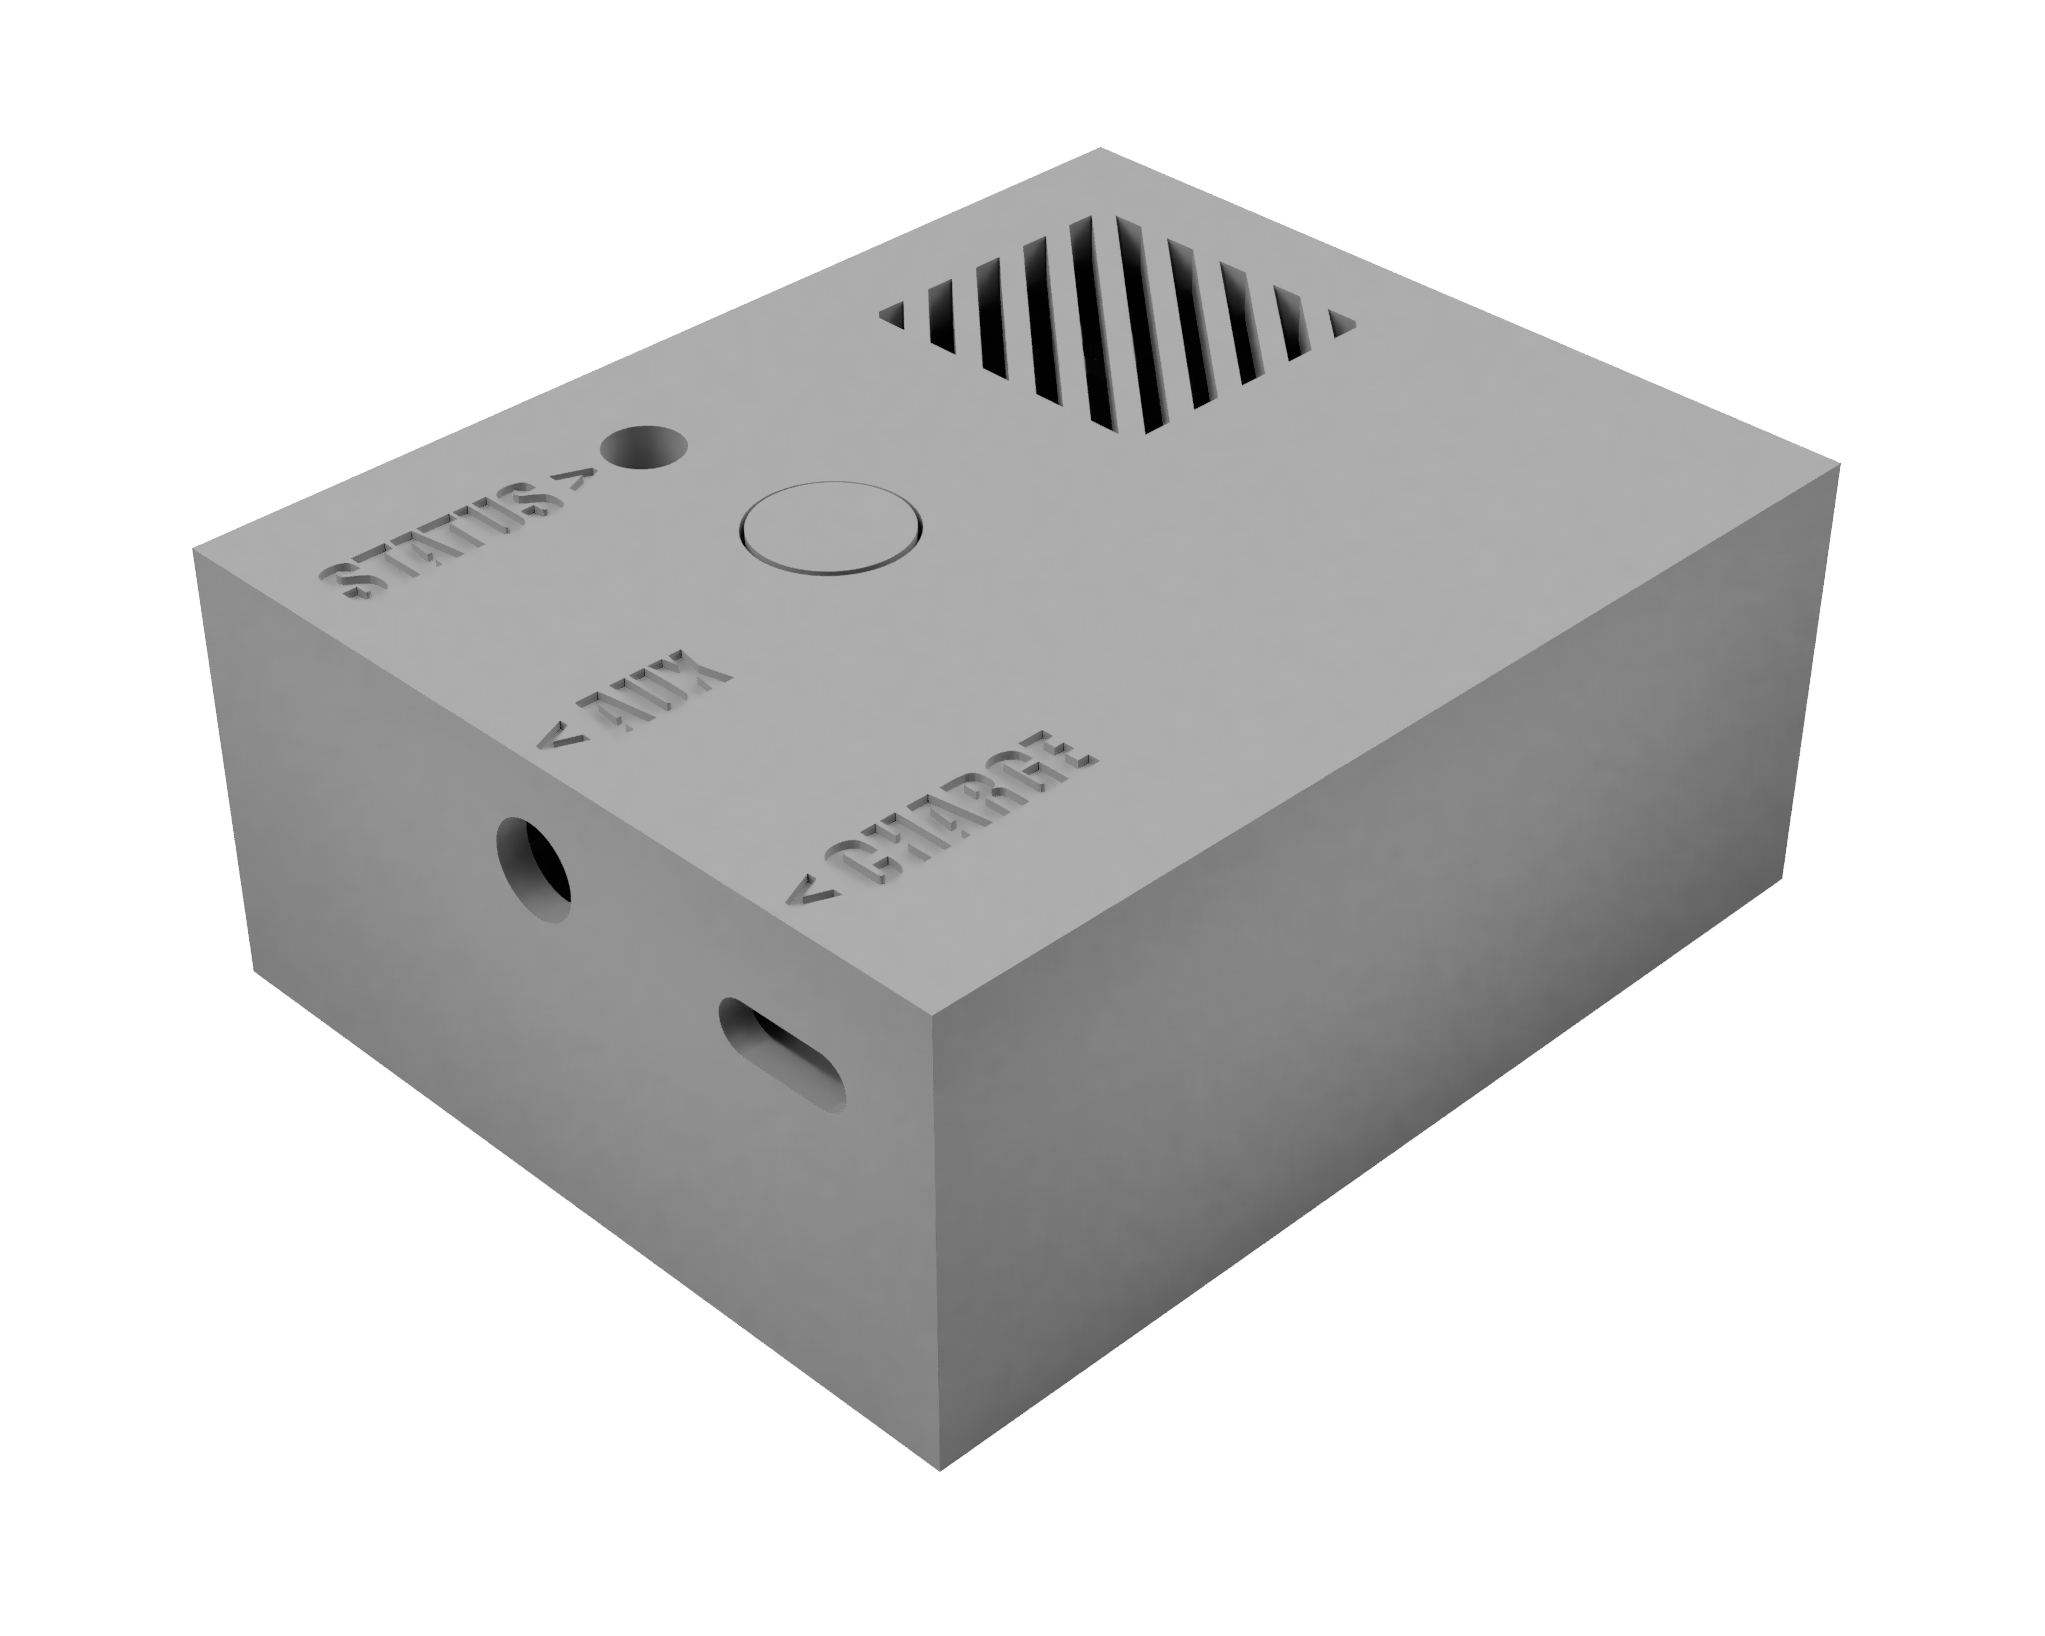
\includegraphics[scale=0.18]{/hardware/adapter-nahe_hg-transparent.png}
\end{center}
\end{figure}

\pagebreak

\section{Projekt}
\subsection{Projektteam}
\textbf{Nico Lang}\\
Wirtschaftsingenieure/Betriebsinformatik\\
Grießau\\
6651 Häselgehr AT\\
Nico.Lang@hak-reutte.ac.at\\
\\
\textbf{Philipp Immler}\\
Wirtschaftsingenieure/Betriebsinformatik\\
Hoheneggweg 21a\\
6682 Vils AT\\
Philipp.Immler@hak-reutte.ac.at

\pagebreak

\subsection{Eidesstattliche Erklärung}
Hiermit versichere ich, dass ich die vorliegende Arbeit selbstständig verfasst und keine anderen Hilfsmittel als die angegebenen benützt habe. Die Stellen, die anderen Werken (gilt ebenso für Werke aus elektronischen Datenbanken oder aus dem Internet) wörtlich oder sinngemäß entnommen sind, habe ich unter Angabe der Quelle und Einhaltung der Regeln wissenschaftlichen Zitierens kenntlich gemacht. Diese Versicherung umfasst auch in der Arbeit verwendete bildliche Darstellungen, Tabellen, Skizzen und Zeichnungen. Für die Erstellung der Arbeit habe ich auch folgende Hilfsmittel generativer KI-Tools (ChatGPT 3.5) zu folgendem Zweck verwendet: Inspiration und allgemeine Information. Auch Übersetzer (DeepL) wurden zur Hilfe genommen. Die verwendeten Hilfsmittel wurden vollständig und wahrheitsgetreu inkl. Produktversion und Prompt ausgewiesen.\\

\vspace{30mm}

\noindent
\begin{minipage}[c]{5cm}
	\centering \dotfill \\
	Ort, Datum
\end{minipage}
\hfill
    \begin{minipage}[c]{5cm}
        \centering \dotfill \\
        Unterschrift Schüler/in
    \end{minipage}
    
\vspace{10mm}

\noindent
\begin{flushright}
    \begin{minipage}[c]{5cm}
        \centering \dotfill \\
        Unterschrift Schüler/in
    \end{minipage}
\end{flushright}

\pagebreak

\subsection{Abstract Deutsch}
Die vorliegende Diplomarbeit beschäftigt sich mit der Entwicklung eines Multi-Room Sound Adapters. Ein einzelner Adapter besitzt dabei die Funktion, einen Audiostream aus dem Internet auf einen Line-Output auszugeben. So lassen sich die Adapter beispielsweise mit aktiven Lautsprechern per Klinkenkabel verbinden, um so Musik in voneinander getrennten Räumen abzuspielen. Welche Musik in welchem Raum spielt, ist frei konfigurierbar. Dabei erfolgt die Konfiguration per Smartphone-App. Das Endergebnis der Diplomarbeit sind somit der Adapter selbst (physischer Prototyp) und die dazugehörige Smartphone-App. \newline \\
Die Diplomarbeit lässt sich grob in die drei Teile Planung, Entwicklung und Testen/Fehlerbehebung gliedern.
\subsection{Abstract English}
This diploma thesis deals with the development of a multi-room sound adapter. A single adapter has the function of outputting an audio stream from the Internet to a line output. For example, the adapters can be connected to active speakers via a jack cable in order to play music in separate rooms. Which music plays in which room is freely configurable. The configuration is done via smartphone app. The final result of the thesis is the adapter itself (physical prototype) and the corresponding smartphone app. \newline \\
The thesis can be roughly divided into three parts: planning, development and testing/troubleshooting.
\subsection{Danksagung}
Wir bedanken uns bei den betreuenden Lehrpersonen Dipl. Ing. Dr. Peter L. Steger und Dipl. Päd. Johannes Köll für die kompetente Unterstützung.

\pagebreak
\tableofcontents
\pagebreak

\section{Einleitung}
\begin{figure}[H]
\begin{center}
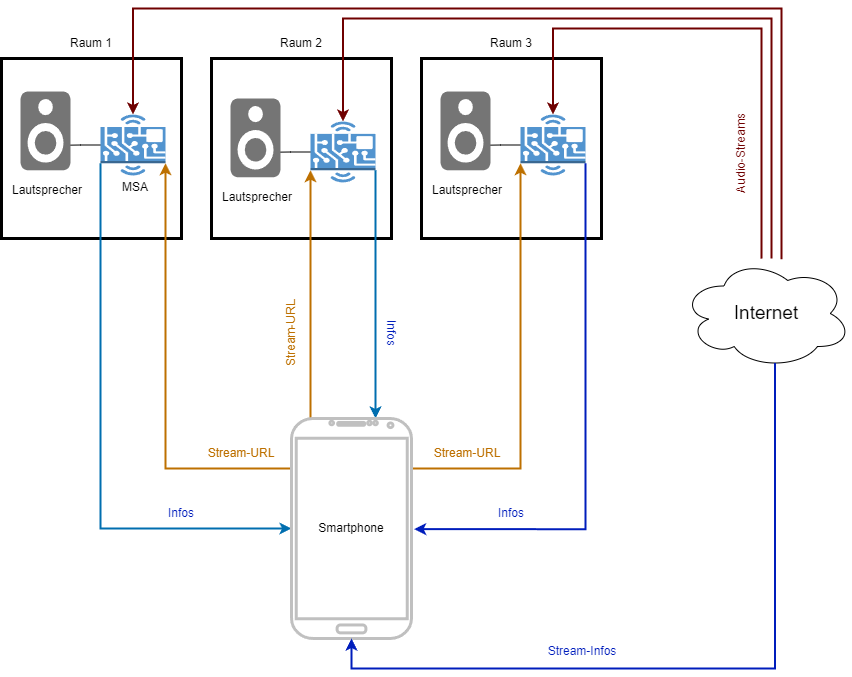
\includegraphics[scale=0.8]{/allgemein/MSA_Konzept.png}
\caption{Skizze Gerätekette}
\end{center}
\end{figure}
Hier ist eine vereinfachte Darstellung der Gerätekette und wie sich der Multi-Room Sound Adapter in diese eingliedern lässt.\newline
Am unteren Bildrand ist eine Wolke mit Information dargestellt. Sie symbolisiert das Internet mit dessen Inhalt. Darüber ein Smartphone, welches mit dem Internet kommuniziert und sich so Informationen wie Stream-URLs holt und sie an den Adapter weitergibt. Der Adapter selbst (hier als blaue Platine dargestellt) holt sich den Stream selbst (also praktisch ein Audiosignal) und stellt ihn als Klinkenausgang zur Verfügung. Man kann diesen dann beispielsweise mit einem Lautsprecher verbinden und Musik hören.

\subsection{Einleitung Hardware}
Das Ziel des Hardware-Teils für folgende Diplomarbeit war, einen sinnvollen internen Aufbau des Geräts zu erzielen, die am besten geeigneten Hardware-Komponenten zu finden, das System bzw. die einzelnen Komponenten zusammenzusetzen und zu testen. Dieser Teil der Diplomarbeit wird von Nico Lang übernommen.
Zudem beschäftigt sich dieser Teil mit dem Gehäuse des Geräts und bestimmt die technischen Anforderungen (Schnittstellen), die der Adapter letztendlich haben soll. 
Bei der Planung soll zudem darauf geachtet werden, möglichst viele Kosten einzusparen, ohne dabei die Faktoren der Sicherheit und Qualität zu vergessen.

\subsection{Einleitung Software}
Das Ziel des Software-Teils für folgende Diplomarbeit war, einerseits die Software des Adapters, andererseits die Software der Smartphoneapp zu entwickeln. Dieser Teil der Diplomarbeit wurde von Philipp Immler übernommen. Die Software des Adapters wurde mit der Programmiersprache C++ codiert. Die Software der Smartphoneapp wurde mit JavaScript codiert. Bei der Programmierung wurden zahlreiche Bibliotheken und Frameworks verwendet. Dies hat den Vorteil, dass diese schon vorgefertigte Lösungen für bestimmte Probleme bieten und man deshalb nicht alles von Grund auf neu entwickeln muss. 

\section{Planung}
\subsection{Festlegung Funktionsweise}
Beim Festlegen einer grundlegenden Funktionsweise des Adapters stellen sich vor allem folgende Fragen:
\subsubsection{Was soll das System können?}
Das Hauptziel ist, dass das System in verschiedenen, voneinander getrennten Räumlichkeiten bestimmte Audiosignale auf einen Line-Ausgang abspielen kann.
\vspace{4mm}\newline
\textbf{Line-Ausgang}\newline
Ein Line-Ausgang (Line-Out) ist eine Ausgangs-Schnittstelle für analoge Audiosignale, deren Ausgangsspannung immer grob dem Line-Pegel entspricht. Dieser \glqq Line-Pegel beträgt etwa 0,5 Volt bis 1 Volt\grqq{}. \newline
Diese geringe Spannung reicht jedoch nicht, um das Audio-Signal direkt an einen Lautsprecher auszugeben. Es muss zuerst noch durch einen Verstärker verstärkt werden. Lautsprecher gibt es mit eingebautem Verstärker (aktive Lautsprecher), es gibt sie jedoch auch ohne internen Verstärker (passive Lautsprecher).
\vspace{4mm}\newline
(vgl. \url{https://www.monacor.de/magazin/audio-pegel})
\vspace{4mm}\newline
\textbf{Aktive vs. Passive Lautsprecher}\newline
Ein klassisches Beispiel für passive Lautsprecher sind herkömmliche Hi-Fi Stereoanlagen. Diese bestehen meistens aus einem oder mehreren Playern, einem Verstärker und zwei oder mehreren (Surround Sound also Raumklang) passiven Lautsprechern. Der Player liest das Signal (beispielsweise einer CD oder einer Schallplatte) und gibt den Line-Pegel über ein Kabel (im Hi-Fi Bereich meist Cinch oder 3,5mm Klinke) an den Verstärker weiter. Dieser Line-Pegel kann aber auch direkt aus einem TV-Gerät oder wie in unserem Fall aus einem Multi-Room Sound Adapter kommen. Der Verstärker verstärkt das Audiosignal nun von der geringen Spannung des Line-Pegels auf die für die Lautsprecher passende Spannung. Mit dem Lautstärkeregler am Verstärker kann man sich die Spannung (also Lautstärke) letztendlich noch auf persönliche Präferenzen anpassen. \newline
Ein Beispiel für aktive Lautsprecher sind Bluetooth-Lautsprecher, deren Hauptziel es ist, möglichst kompakt und leicht transportierbar zu sein. Solche Bluetooth-Lautsprecher enthalten im Normalfall einen Akku, um auch unterwegs, ohne aktive Stromquelle, Musik hören zu können. Somit enthält das Gehäuse den Verstärker, die Lautsprecher, den Akku und sonstige Elektronik wie unter anderem ein Bluetooth-Modul. Hier fungiert meist ein herkömmliches Smartphone als Signalgeber, ob über Bluetooth oder 3,5mm Klinke bleibt dem/der Benutzer/-in überlassen.\newline
Lenovo beschreibt Line-Ausgänge zum Beispiel folgendermaßen: \glqq Der Line-Ausgang unterscheidet sich von anderen Audioausgängen wie z. B. Kopfhörerbuchsen, da er ein Signal mit festem Pegel liefert, das nicht von der Lautstärkeregelung Ihres Geräts beeinflusst wird. Er ist für den Anschluss an Geräte gedacht, die das Audiosignal verstärken oder weiterverarbeiten können.\grqq{} \newline
Man kann also daraus schließen, dass man das Line-Out Signal des Multi-Room Sound Adapter vor dem Lautsprecher noch verstärken muss. Wie genau, ist dem/der Endverbraucher/-in überlassen.
\vspace{4mm} \newline
(vgl. \url{https://www.lenovo.com/at/de/glossary/line-out})
\vspace{4mm}\newline
\textbf{Audioqualität}\newline
Zudem ist es wichtig, dass das System den Ton zuverlässig und möglichst flüssig überträgt und ausgibt.\newline
\glqq Das menschliche Ohr ist theoretisch in der Lage, Frequenzen von 20 Hz bis 20 kHz zu hören. Die
Obergrenze von 20 kHz nimmt mit dem Alter ab. \grqq{} \newline
Es gibt drei wichtige Grundgrößen wenn es um Audioqualität geht: Samplerate, Auflösung und Bittiefe. Jan Baumann hat diese auf seiner Website sehr gut erklärt:
\vspace{4mm}\newline
\glqq Die \textbf{Samplerate} (Einheit Hz = Hertz) gibt an, wie oft in einer Sekunde der Audio-Pegel erfasst und gespeichert wird. Eine Angabe von 44.100 Hz (44,1 kHz) bedeutet, dass 44.100 Werte für eine Sekunde Musik gespeichert werden. Übliche Sample-Raten sind 44,1 kHz (Musik CD), 48 kHz (Film) und 96 kHz (Tonstudio). \grqq{}
\vspace{4mm}\newline
\glqq Die \textbf{Auflösung} (Einheit Bit) gibt an, wie viel Speicher für so einen Sample-Wert genutzt wird. Zum Beispiel erlauben 16 Bit (2-hoch-16) eine Skala von 65.536 Werten für jeden einzelnen Sample-Wert. Wenn wir viel Speicher für einen Wert haben, können wir das Signal also mit mehr Genauigkeit verarbeiten. Übliche Werte sind 16 Bit (Musik CD) oder 24 Bit bzw. 32 Bit im Studio.\grqq{}
\vspace{4mm}\newline
\glqq Die \textbf{Bitrate} bzw. Datenrate (kBit/s) wird oft mit der Auflösung verwechselt. Sie steht für die “Bandbreite” der Audiodatei, also welche Datenmenge in einer Sekunde verarbeitet wird. Für unkomprimierte Formate wie WAV und AIFF berechnet man die Bitrate ganz einfach, indem man die drei Werte von oben multipliziert: \grqq{}\newline
Mehr zu Audioqualität aber im Teil "Auswahl interne Hardware/Digital-/Analogwandler"
\vspace{4mm} \newline
(vgl. \url{https://www.axis.com/dam/public/ad/35/af/einf%C3%BChrung-in-das-thema-audio:-akustik-,-lautsprecher-und-audio-terminologie-de-DE-191125.pdf}) 
\newline
(vgl. \url{https://www.baumannmusic.com/de/2012/sampleratehz-und-khz-aufloesung-bit-und-bitrate-kbits/}
\vspace{4mm}\newline
\textbf{Audio-Quellen}\newline
Grundsätzlich kann jeder beliebige Audio-Stream aus dem Internet verwendet werden. Das können beispielsweise Radiosender sein.
Ein Beispiel für einen solchen Audio-Stream wäre der, des österreichischen Radio-Senders \glqq OE3\grqq{}: \newline
\url{https://orf-live.ors-shoutcast.at/oe3-q2a}
\vspace{4mm}\newline
\textbf{Benutzerfreundlichkeit}\newline
Es wird zudem viel Wert auf Benutzerfreundlichkeit gelegt. Das bedeutet, dass sich der Adapter zum einen leicht einrichten lässt, aber auch, dass er sich (mithilfe der Smartphone-App) einfach bedienen lässt.
\vspace{4mm} \newline
(vgl. (Fachbuch) \url{https://books.google.de/books?id=UI2INugaKwIC&pg=PA219#v=onepage})
\subsubsection{Was muss es nicht können?}
Dieser Multi-Room Sound Adapter ist als Hi-Fi Produkt für den klassischen Durchschnittsbürger und/oder Musik-Liebhaber gedacht. Aufgrund dessen wurde die Bedienung sehr einfach und benutzerfreundlich, jedoch eindeutig nicht so präzise oder vielfältig einstellbar gestaltet wie es bei professionellem Audio-Equipment der Fall ist. Während der Laie das Produkt einfach anstecken und benutzen möchte, hätte ein Audio-Nerd beispielsweise gerne noch einen eingebauten Acht-Band Equalizer und vieles mehr. Das war jedoch nicht das Ziel dieser Diplomarbeit. Es ging eher darum, die Hauptfunktion, also Ton kabellos in Räume zu übertragen, und Einstellungsmöglichkeiten per App ohne großes Kopfzerbrechen zu ermöglichen.\newline
Wie schon oben erwähnt liefert der Multi Room Sound-Adapter nur einen Audioausgang mit Line-Pegel und es ist ihm nicht möglich, dieses zu verstärken. Man kann also keine Kopfhörer mit einer Impedanz über 80 Ohm direkt an das Gerät anschließen (man kann theoretisch schon, aber der Ton wird sehr leise sein). Das Audiosignal muss also zuerst mit einem Verstärker verstärkt werden.\newline
\subsubsection{Wie könnte man es erweitern?}
Unsere Variante des Multi-Room Sound Adapter zeichnet sich vor allem durch die beliebige Erweiterbarkeit aus. In der Theorie soll es ein einzelnes Modell, also den Adapter selbst geben. Mit jedem weiteren Adapter kann dementsprechend ein weiterer Lautsprecher oder ein Raum zugefügt werden. In Zukunft wäre es auch vorstellbar, dass man aus mehreren Adaptern Gruppen bilden kann, in denen die Adapter synchronisiert sind und somit der gleiche Audio-Stream auf mehreren Adaptern synchron läuft. Dies ist aber technisch sehr aufwendig, da die Latenz von WiFi ziemlich hoch ist.\newline

SKIZZE: Grundriss mit Lautsprechern in allen Räumen und Gruppenbildung
\subsection{Auswahl Hardwarekomponenten}
Zur Auswahl der Hardwarekomponenten des Adapters wurde zu aller erst die externe Ausstattung des Adapters überlegt. Das bedeutet praktisch alles, mit dem ein Endverbraucher letztendlich zu tun hat. Dann kann der interne Teil, also die Technik dahinter, individuell auf die Anforderungen des externen Teils designet und entwickelt werden.
\subsubsection{Auswahl externe Hardware}
Der Adapter sollte ein möglichst kompakt konstruiertes und stabiles Gehäuse bekommen. An diesem ist ein einfacher Taster zur Interaktion angebracht. Mit dem Taster sind einige Funktionen des Adapters ermöglicht. Beispielsweise per Klick, Doppelklick oder kurzem Halten. Da sich die Aufgaben des Tasters selbst gering halten (Verbindungsvorgang, Ein- und Ausschalten, ...) wurde nur ein einziger Taster verwendet, um die Komplexität des Gesamtsystems zu senken. Die weitaus komplizierteren Funktionen wurden alle samt in der Smartphone-Applikation ermöglicht. Zusätzlich wurde eine RGB-Leuchtdiode zur Statusanzeige verbaut, um beispielsweise den aktuellen Verbindungsstatus zum Mobilgerät und zum Internet anzuzeigen. \newline \\
\textbf{Gehäuse} \newline
Das Gehäuse soll alle Komponenten auf möglichst kleinem Raum zusammenhalten, schützen und kühlen. Da sich Komponenten und möglicherweise auch das Design selbst laufend änderten, wurde dieses erst gegen Ende des Projekts finalisiert. Mehr dazu im Teil "Design Adaptergehäuse". \newline \\
\textbf{Taster} \newline
Für den Taster wurde ein herkömmlicher Tactile-Button mit verlängertem Taster in das Gehäuse geplant. Auf ihm klebt eine Art Aufsatz, auf den der/die Endverbraucher/-in letztendlich drückt, um ein gleichbleibendes optisches Design des Gehäuses zu ermöglichen. Mehr dazu im Teil "Design Adaptergehäuse"\newline \\
\textbf{LED (Light-Emitting Diode)} \newline
Als Statusanzeige wurde in diesem Fall eine herkömmliche RGB-LED verwendet. Mit dieser ist es theoretisch möglich, alle Farben des RGB-Spektrums (16,7 Mio) mit einer Komponente darzustellen.\newline
Man muss sich jedoch im klaren darüber sein, für wie viel Spannung die benutzte LED gebaut ist. Dann kann man mit passenden Widerständen arbeiten, um die LED nicht aufgrund zu hoher Spannung zu beschädigen.
\vspace{4mm} \newline
(vgl. \url{https://www.elektronik-kompendium.de/sites/praxis/bauteil_rgb-led.htm})
\subsubsection{Auswahl interne Hardware}
\textbf{Mikrocontroller (ESP32)}\newline
Als Herz des Systems wird ein ESP32-WROOM-32 Mikrocontroller mit angebauter Platine (DOIT ESP32 DEVKIT V1) verwendet. Der ESP32 ist ein weit verbreiteter Mikrocontroller. Das Konzept des Controllers sind GPIOs (general purpose input/output) also Pins die man mit Code mit bestimmten Funktionen beschreiben kann. Man kann die Arduino IDE mit C++ als Programmiersprache zum programmieren verwenden. Zudem verfügt er schon Onboard über einen Hybrid WIFI- und Bluetooth-Chip, wodurch externe Module vermieden, und somit Platz eingespart werden kann. Espressif selbst beschreibt den ESP32 als optimal für IoT-Anwendungen; auch wegen der hohen Energieeffizienz.\newline
Hier ein paar Grundfakten des ESP32-WROOM-32 (der Controller selbst):\newline
Der von uns benutzte ESP32 hat einen Dual-Core 32-bit Prozessor (2x Tensilica-LX6-Kernen). Der Mikrocontroller hat WLAN (802.11b/g/n) und kann ein eigenes WLAN Netzwerk (Access Point) erstellen (kleiner WebServer). Er unterstützt Bluetooth 4.0 (BLE/Bluetooth Smart) und Bluetooth Classic. Dies ist bei vielen SmartHome und IoT-Anwendungen nützlich. Er hat einen geringen Stromverbrauch von 50-70 mA (kleine Programme ohne WiFi). Der Deep-Sleep Modus macht einen Stromverbrauch von unter 0,1mA möglich. Die Anschaffungskosten fallen mit unter 10 Euro im Vergleich zu anderen Mikrocontrollern auch sehr niedrig aus.\newline
Wie schon erwähnt ist der ESP32 mit der (uns vertrauten) Arduino IDE programmierbar und kann auch in industriellen Umgebungen (-40°C bis +125°C) betrieben werden.\newline
Für den Multi Room Sound-Adapter kommt ein ESP32 Entwicklungsboard (DOIT ESP32 DEVKIT V1) zum Einsatz.\newline
Hier eine Beschreibung von Dev-Kits auf digitalewelt.at: \glqq Um alle Funktionen des ESP32 Moduls einfach nutzen zu können, gibt es sogenannte Entwicklungsboards. Diese sind nicht nur mit zusätzlichen Schaltungen für die Spannungsversorgung ausgestattet, sondern bieten uns auch die gängigen Anschlussmöglichkeiten für unsere externen Komponenten.\grqq{} \newline
Erwähnenswert ist auch, dass der ESP32 an manchen GPIOs intere Pullup- /Pulldown-Widerstände hat. \glqq Wenn man einen Pin, an dem z.B. ein Sensor hängt, mit pinMode(5, INPUT) konfiguriert, hat der Pin keinen definierten Pegel.
Aus diesem Grund kann er solange zwischen HIGH und LOW schwanken, bis ihm ein Zustand zugeschrieben wird. \grqq{} ... \glqq Dafür hat der ESP32 interne Pullup- / Pulldown-Widerstände, die zugeschaltet werden können. Diese können mit INPUT\_PULLUP als Argument im Befehl pinMode() eingeschaltet werden.
Bei INPUT\_PULLUP wird der Pin als Eingang deklariert und wenn er nicht beschaltet ist wird dieser auf HIGH gesetzt.
Bei INPUT\_PULLDOWN hingegen wird der Eingang auf LOW gesetzt.\grqq{} Pullup- /Pulldown-Widerstände sind essenziell für einen sauber konfigurierten Tactile-Button.
\vspace{4mm} \newline
(vgl. \url{https://www.espressif.com/en/products/socs/esp32}) \newline
(vgl. \url {https://digitalewelt.at/esp32-grundlagen/})\newline
(vgl. \url {https://www.xplore-dna.net/mod/page/view.php?id=2741&forceview=1}
\vspace{4mm}\newline
\textbf{Digital-/Analogwandler (Audio-Modul)}\newline
Dieses Modul ist ausschlaggebend für eine gute Audioqualität. Das digitale Audiosignal vom ESP32 (Radiostream) muss nämlich für die Line-Out Buchse auf analog konvertiert werden. Dafür wird ein Modul mit dem PCM5102A (\glqq 2VRMS DirectPath™, 112 dB Audio Stereo DAC mit 32-bit, 384 kHz-PCM-Schnittstelle\grqq{}) DAC verwendet. Auf diesem Modul befinden sich alle Komponenten sowie die Klinkenbuchse die für die Ausgabe des Audiosignals nötig sind.
\vspace{4mm} \newline
(vgl. \url{https://www.ti.com/product/de-de/PCM5102A})
\vspace{4mm}\newline
\textbf{Akku (Li-Ion)}\newline
Das Endprodukt soll mithilfe eines Akkus auch ohne Strom auskommen, dafür wird ein Lithium-Ionen-Akku mit 3,7 Volt verwendet. Akkus dieser Art zeichnen sich durch ihre hohe Energiedichte und, unter guten Umständen, hohe Lebensdauer aus. Man verwendet Li-Ionen-Akkus meist für (tragbare) Geräte in denen andere Akkus zu schwer oder zu groß wären. (vgl. \url{https://www.chemie.de/lexikon/Lithium-Ionen-Akkumulator.html}) \vspace{4mm}\newline
Natürlich haben Li-Ionen-Akkus auch gewisse Nachteile und bergen wie jeder andere Akku Gefahren. Beispiele dafür sind elektrische Überlastung, mechanische Beschädigung und thermische Überlastung:

Eine elektrische Überlast kann etliche Gründe haben, darunter: 
\begin{itemize}
	\item Verwendung eines falschen Ladegerätes
	\item Tiefenentladung
	\item Falsche Lagerbedingungen (z.B.: zu hohe Temperaturen) 
\newline
Zitat: \glqq Hier kommt es zur Zersetzung der Elektrolytflüssigkeit und infolgedessen zur Bildung leicht brennbarer Gase. Wird anschließend versucht, die tiefentladenen Lithium-Ionen-Zellen wieder aufzuladen, kann die zugeführte Energie durch das Fehlen von Elektrolytflüssigkeit nicht mehr korrekt umgesetzt werden. Es kann zum Kurzschluss beziehungsweise zum Brand kommen.\grqq{} (vgl. \url{https://www.denios.de/services/denios-magazin/gefahren-im-umgang-mit-lithium-ionen-akkus})
\end{itemize}
Eine mechanische Beschädigung jeglicher Art kann zu Kurzschlüssen im inneren der Zelle führen. Da unser Gerät nicht dafür gemacht ist, ständig in Bewegung zu sein, spielt dies keine zu große Rolle, es muss jedoch trotzdem ausreichend Schutz gegeben sein, was durch das Gehäuse sichergestellt wird.
\vspace{4mm}\newline
Wie oben schon kurz erwähnt, muss großer Wert auf die richtige Lagerung/Kühlung des Akkus gelegt werden. Wird dieser zu heiß (etwa durch den Mikrocontroller oder sonstige Bauteile) oder durch äußere Einflüsse beschädigt kann es zum Brand kommen.
\vspace{4mm}\newline
Man kann daraus schließen, dass jeder kleinste Fehler beispielsweise zu einem Brand oder sogar einer Explosion des Akkus führen kann. Es ist daher wichtig, den Akku mit absoluter Vorsicht zu handhaben. Ausreichend Tests (Betriebstemperatur, etc.), richtige Konfiguration des Ladereglers und die Auswahl des Akkus sind ausschlaggebend für die Sicherheit des Endverbrauchers und dessen Umfeld.

(vgl. \url{https://www.denios.de/services/denios-magazin/gefahren-im-umgang-mit-lithium-ionen-akkus})

\textbf{Laderegler}\newline
Für einen optimalen Ladeprozess und Schutz des Akkus wird ein spezieller Laderegler verwendet. Dieser regelt somit den Ladevorgang des Akkus und hört auf zu laden, sobald dieser voll ist. Der Aufbau dieses Ladereglers ist nicht kompliziert, es gibt jeweils einen Plus- und Minuspol für den Eingang (USB-C Buchse), den Akku (im englischen auch als Battery bezeichnet) und den Ausgang.
\subsection{Auswahl Technologien}
\subsubsection{Protokolle}
In diesem Kapitel geht es um die Recherche und Auswahl von Protokollen, die für den Austausch von Daten verwendet wurden.
\newline \\
\textbf{HTTP} \\
Das Hyper Text Transfer Protocol ist ein weitverbreitetes Protokoll im Web und wird größtenteils für die Kommunikation zwischen Browsern und Webservern eingesetzt. Dabei basiert das Protokoll auf sogenannten \glqq Requests\grqq{} (auf Deutsch: Anfragen). Es gibt zahlreiche Anwendungen für HTTP. Wir nutzen es einerseits für die Kommunikation zwischen Smartphoneapp (Client) und Microcontroller (Server) mittels REST-API und zum Empfangen der Audio-Streams. (vgl. URLPI02) \newline \\
\textbf{I2S}\\
Das Inter IC Sound Protocol wird verwendet, um Stereo-Audio-Daten zwischen ICs auszutauschen. Es benötigt für die Datenübertragung folgende Leitungen:
\begin{itemize}
\item Taktleitung
\item Wortauswahl
\item mindestens eine Datenleitung
\end{itemize}
Die Datenübertragung erfolgt seriell und synchron. Seriell bedeutet, dass die Daten nur durch eine Leitung (die Datenleitung), nacheinander übertragen werden. Synchron bedeutet, dass die Daten in einem bestimmten Takt übertragen werden. Dieser Takt wird von der Taktleitung vorgegeben. Die Leitung für die Wortauswahl wählt den Stereokanal aus (links oder rechts). (vgl. URLPI12) \\
In unserem Projekt wurde das I2S Protokoll verwendet, um die digitalen Stereo-Audio-Daten vom Microcontroller an den Digital-Analag-Wandler zu übertragen.
Dabei werden die Buffer, die der Microcontroller vom Audio-Stream erhält, mittels I2S an den Digital-Analog-Wandler gesendet, welcher die digitalen Daten in analoge PCM (Pulse Code Modulation) Daten umwandelt, so dass diese dann anschließend auf der Lautsprecherbox ausgegeben werden können.
\subsection{Auswahl Softwaretools}
\subsubsection{Einleitung}
In diesem Kapitel geht es um die Recherche und Auswahl von geeigneten Softwaretools, welche für die App-Entwicklung, als auch für die Entwicklung der Software des Microcontrollers verwendet wurden. Zusätzlich werden auch die Softwaretools, welche zum Schreiben dieser Diplomarbeit verwendet wurden, kurz beschrieben. 
\vspace{4mm}\newline
\textbf{LaTeX} \\
"LaTeX ist ein hochwertiges Schriftsatzsystem, das Funktionen für die Erstellung technischer und wissenschaftlicher Dokumentationen enthält. LaTeX ist der De-facto-Standard für die Kommunikation und Veröffentlichung von wissenschaftlichen Dokumenten." (Übersetzung des englischen Originals von: https://www.latex-project.org/) \\
Wir haben uns für das Schreiben unserer Diplomarbeit in LaTeX entschieden, weil es sich sehr gut für wissenschaftliche Arbeiten eignet und wir somit schon damit vertraut sind, wenn wir es in der Zukunft, zum Beispiel im Studium benutzen müssen.
\vspace{4mm}\newline
\textbf{draw.io}
"draw.io ist eine kostenlose Online-Diagrammsoftware zur Erstellung von Flussdiagrammen, Prozessdiagrammen, Organigrammen, UML, ER und Netzwerkdiagrammen." (Übersetzung des englischen Originals von: https://app.diagrams.net/) \\
Wir haben alle Diagramme, welche in unserer Diplomarbeit zu sehen sind, in draw.io erstellt, weil es einfach zu handhaben ist und es eine große Auwahl an Diagrammtypen und Formen bereitstellt.
\vspace{4mm}\newline
\textbf{Visual Studio Code} \\
"Visual Studio Code ist ein leichtgewichtiger, aber leistungsstarker Quellcode-Editor, der auf Ihrem Desktop läuft und für Windows, macOS und Linux verfügbar ist. Er bietet integrierte Unterstützung für JavaScript, TypeScript und Node.js und verfügt über ein umfangreiches Ökosystem von Erweiterungen für andere Sprachen und Laufzeiten (wie C++, C\#, Java, Python, PHP, Go, .NET)." (Übersetzung des englischen Originals von: https://code.visualstudio.com/docs) \\
Wir haben Visual Studio Code als IDE für unsere Diplomarbeit gewählt, weil durch die unzähligen Erweiterungen viele verschieden Programmiersprachen und Bibliotheken unterstützt werden und wir somit den gesamten Code, sowohl für den Microcontroller als auch für die Smartphoneapp, darin schreiben konnten.
\vspace{4mm}\newline
\textbf{GitHub} \\
"GitHub ist eine webbasierte Schnittstelle, die Git verwendet, die Open-Source-Software zur Versionskontrolle, mit der mehrere Personen gleichzeitig separate Änderungen an Webseiten vornehmen können. Wie Carpenter anmerkt, fördert GitHub die Zusammenarbeit von Teams bei der Erstellung und Bearbeitung von Website-Inhalten, da es eine Zusammenarbeit in Echtzeit ermöglicht." (Übersetzung des englischen Originals von: https://digital.gov/resources/an-introduction-github/) \\
Wir verwenden GitHub für die Verwaltung unseres Codes und unserer Dokumente. Der Vorteil dabei ist, dass jedes Projektmitglied auf seinem lokalen PC an den Dokumenten arbeiten kann und die Änderungen dann per GitHub synchronisiert werden.
\vspace{4mm}\newline
\textbf{DeepL} \\
Wir verwenden DeepL um englische Texte, welche für unsere Diplomarbeit relevant sind, ins Deutsche zu übersetzen. Wir haben uns für DeepL entschieden weil dieser einer der genauesten Übersetzer, dank integrierter KI, ist und man diesen außerdem kostenlos nutzen kann.
\subsubsection{Bibliotheken Microcontroller}
Im folgenden werden die verwendeten Bibliotheken im Code des Microcontrollers aufgezählt und kurz beschrieben:
\vspace{4mm}\newline
\textbf{arduino-esp32} \\
(https://github.com/espressif/arduino-esp32) \\
Die arduino-esp32-Bibliothek wurde verwendet um den ESP32 ähnlich wie einen Arduino programmieren zu können. Es erleichtert dabei die Programmierung enorm, vorallem dann, wenn man schon Vorerfahrung mit der Programmierung von Arduinos hat. Ein weiterer Vorteil ist, dass diese Bibliothek bereits weitere nüztliche Bibliotheken beinhaltet, welche für die Programmierung benötigt werden.
\vspace{4mm}\newline
\textbf{WiFi} \\
(https://github.com/espressif/arduino-esp32/tree/master/libraries/WiFi) \\
Die WiFi-Bibliothek ist eine offizielle Bibliothek von Arudino, welche ebenfalls in der arduino-esp32-Bibliothek inkludiert ist. Sie wird verwendet, um die Funktionen der eingebauten WiFi-Antenne des ESP32 zu verwenden. Der ESP32 kann dabei entweder als Access Point oder als Client fungieren. Wenn er als Access Point fungiert, stellt er ein eigenes WiFi-Netzwerk bereit, mit dem sich andere Geräte verbinden können und der ESP32 somit einen Host darstellt. Als Client kann er sich mit anderen WiFi-Netzwerken bzw. Access Points verbinden. In unserem Projekt fungiert der ESP32 sowohl als Access Point, als auch als Client.
\vspace{4mm}\newline
\textbf{ArduinoJson} \\
(https://github.com/bblanchon/ArduinoJson) \\
Die ArduinoJson-Bibliothek wird verwendet, um Daten in das JSON-Format zu kodieren. JSON (Java Script Object Notation) ist ein Datenformat, welches oft für den einheitlichen Datenaustausch zwischen Server und Client verwendet wird. Dabei verwendet JSON sogenannte Schlüssel-Wert-Paare. Das heißt, ein Wert hat immer einen eindeutigen Schlüssel. In unserem Projekt wird die ArduinoJson-Bibliothek für den einheitlichen Datenaustausch zwischen Webserver (ESP32) und Client (Smartphone) verwendet. (vgl. URLPI11)
\vspace{4mm}\newline
\textbf{WebServer} \\
Die WebServer-Bibliothek wird verwendet, um einen Webserver auf dem ESP32 bereitzustellen. Dieser ist wichtig für die Funktion als REST-API und somit für den Datenaustausch zwischen ESP32 und Smartphoneapp. Der Webserver erhält Anfragen von Clients und sendet diesen dementsprechende Antworten zurück. Dabei gibt es vordefinierte Routen, welche aufrufbar sind.
\vspace{4mm}\newline
\textbf{ESP32-audioI2S} \\
(https://github.com/schreibfaul1/ESP32-audioI2S) \\
Die ESP32-audioI2S-Bibliothek wird verwendet, um die MP3-kodierten Audio-Daten vom HLS-Stream zu empfangen, diese in PCM-Signale umzuwandeln und diese dann an den Digital-Analog-Wandler per I2S-Protokoll zu senden. Der ESP32 verfügt bereits standartmäßig über Funktionen, mit deren Hilfe man Audiodaten mittels I2S übertragen kann. Allerdings sind diese sehr komplex in der Verwendung und Konfiguration. Da die ESP32-audioI2S-Bibliothek bereits die perfekte Lösung für unsere Anforderungen bietet, wurde diese in unserer Diplomarbeit verwendet. \newline \\
\textbf{Preferences} \\
(https://github.com/espressif/arduino-esp32/tree/master/libraries/Preferences)
Die Preferences-Bibliothek wird verwendet, um Schreib- und Lesezugriffe auf den eingebauten EEPROM (Electrical Eresable Programmable Read Only Memory) durchzuführen. Dabei werden die im EEPROM gespeicherten Werte mittels eindeutiger Schlüssel identifiziert.
\subsubsection{Softwaretools Smartphoneapp}
Im foldenden Teil werden die Softwaretools, welche für die Entwicklung der Smartphoneapp verwendet wurden, genauer beschrieben. \\

\textbf{React Native} \\
React Native ist ein Framework, welches die plattformübergreifende Entwicklung von Apps ermöglicht. Das heißt, man schreibt einen Code und kann diesen dann für IOS, Anrdoid und fürs Web verwenden. Der Code wird in JavaScript geschrieben. React Native wurde erstmals 2015 von Meta (damals noch Facebook) als Open-Source-Projekt veröffentlicht. Seither wird es weiterhin von Meta instandgehalten und hat eine riesige Community, welche ständig neue Bibliotheken für das Framewok veröffentlicht. React Native basiert auf React, welches man bereits aus der Webentwicklung kennt. Der Vorteil von React im Gegensatz zur normalen Webentwicklung ist, dass man wiederverwendbare Komponenten bauen kann. Dies ist auch mit React Native möglich. In React Native stehen dabei einige Standardkomponenten zur Verfügung, welche dann jeweils in native Komponenten, passend für das jeweilige Betriebssystem, gerendert werden. 
Wir haben React Native für unsere Smartphoneapp verwendet, weil es sehr aufwendig gewesen wäre, für jede Plattform einen eigenen Code zu schreiben und dies außerdem sehr viel Wissen in unterschiedlichen Bereichen vorausgesetzt hätte. Außerdem hatten wir auch schon etwas Erfahrung mit JavaScript und React, was uns den Einstieg erleichterte.
(vgl. URLPI07)

\textbf{Expo} \\
Um das Entwickeln der Smartphoneapp noch einfacher bzw. effizienter zu gestalten, wurde das Expo Framework verwendet. Dieses Framework basiert auf React Native und stellt noch zusätzlich hilfreiche Bibliotheken und eine Projektstruktur zur Verfügung. Dies hat den Vorteil, dass man bereits den Grundlegenden Aufbau einer App gegeben hat und diesen dann erweitern kann. Ein weiterer Vorteil von Expo ist das File-basierte Routing. Mithilfe diesem ist es möglich, die App-Navigation auf der Ordnerstruktur zu stützen, was die Entwicklung noch einfacher und übersichtlicher macht.
(vgl. URLPI08)

\section{Entwicklung}
\subsection{Entwicklung Software Adapter}
In diesem Kapitel wird der Übergang der Planung in die Entwicklung der Software des Adapters beschrieben. 
Zur Entwicklung der Software des Microcontrollers wurde die IDE Visual Studio Code in Verbindung mit dem Framework PlatformIO verwendet. Um die Entwicklung in C++ zu ermöglichen wurden die bereits erwähnten Bibliotheken verwendet.

\subsubsection{Anforderungen}
Im folgenden wird beschrieben, welche Anforderungen an die Software des Adapters gestellt wurden: \newline \\
\textbf{Access Point} \\
Ein Access Point ist ein Gerät, welches ein WLAN-Netzwerk aufbaut. Dabei können sich WLAN-Clients mit diesem verbinden und somit untereinander Daten austauschen. (vgl. URLPI10)
Der Microcontroller soll im Konfigurationsmodus als Access Point arbeiten. Dies ermöglicht der Smartphoneapp sich als Client zu verbinden und dem Microcontroller mittels HTTP Daten, welche wichtig für die Konfiguration sind (WLAN-Anmeldedaten und Microcontroller-Name), zu senden. \newline \\
\textbf{WLAN Client} \\
WLAN-Clients sind die Geräte, welche mit einem Access Point verbunden sind und somit Teilnehmer in einem WLAN darstellen. Sie können dabei untereinander Daten austauschen.
Wenn der Adapter vollständig konfiguriert ist bzw. alle notwendigen Daten festgelegt sind, soll dieser als WLAN-Client arbeiten. Somit ist es möglich, wenn die Smartphoneapp im gleichen Netzwerk wie der Microcontroller ist, mit diesem zu kommunizieren. Dies geschieht durch die REST-API welche der Microcontroller zur Verfügung stellt. \newline \\
\textbf{REST-API} \\
Der Microcontroller soll eine REST-API zur Verfügung stellen, mithilfe der es möglich ist, per HTTP Daten mit diesem auszutauschen. Eine REST-API ist eine API, welche den Designprinzipien der REST-Architektur folgt. API steht dabei für \glqq Application Programming Interface \grqq{}. Dies ist, wie der Name bereits verrät, eine Schnittstelle von einem Programm. REST steht für \glqq Representational State Transfer \grqq{} und bedeutet so viel wie \glqq repräsentative Zustandsübertragung \grqq{}. Die API muss bestimmte Regeln erfüllen, welche von der REST-Architektur vorgegeben werden. Sie dient dabei zur Kommunikation zwischen Server und Client. Der Client kann mittels HTTP Anfragen an den Server senden. Der Server liefert dann eine Antwort, welche Daten enthalten kann. (vgl. URLPI04) Auf diese Weise kommuniziert die Smartphoneapp mit dem Microcontroller. Der Client kann dabei sogenannte Routen aufrufen. Die aufgerufene Route bestimmt die Aktion, welche auf dem Server aufgerufen wird. Es gibt dabei verschiedene Typen von HTTP-Requests. Jeder Typ is für eine bestimmte Aktion verantwortlich. Die verwendeten Typen in unserem Code sind: GET, POST und PUT. Ein GET-Request wird verwendet, um Daten vom Server abzufragen. Der POST-Request wird verwendet um neue Daten auf dem Server anzulegen. Mit einem PUT-Request werden Daten auf dem Server aktualisiert. (vgl. URLPI13) Im folgenden werden die einzelnen Routen genauer beschrieben: \newline \\
\begin{figure}[H]
\begin{tabularx}{\textwidth}{|l|l|X|}
\hline
\textbf{Route} & \textbf{Anfragen-Typ} & \textbf{Funktion} \\
\hline
/getInfo & GET & Client bekommt die Daten Name, MAC-Addresse, Akkustand, Lautstärke und Stream-URL vom Microcontroller im JSON Format. \\
\hline 
/getAvailableNetworks & GET & Client bekommt eine Liste, gefüllt mit SSID und RSSI (Stärke) von verfügbaren Netzwerken welche sich in der Nähe des Microcontrollers befinden im JSON Format. Diese werden in der Smartphoneapp benötigt, um auszuwählen mit welchem Netzwerk sich der Microcontroller verbinden soll.\\
\hline
/setConfigData & POST & Client sendet SSID und Passwort des gewünschten Netzwerks, sowie Name des Adapters im JSON Format an den Microcontroller. Dieser speichert dann die erhaltenen Daten in den EEPROM und startet neu.\\
\hline
/setStreamUrl & PUT & Client sendet die URL des gewünschten Audio-Streams im Textformat an den Microcontroller. Dieser startet dann den Empfang dieses Streams und gibt diesen auf dem Line-Out aus. \\
\hline
/setVolume & PUT & Client sendet die gewünschte Lautstärke (von 0 bis 100, in Prozent)  des ausgegebenen Audio-Signals als Zahl an den Microcontroller. Dieser legt dann die übertragene Lautstärke beim Audio-Modul fest. \\
\hline
\end{tabularx} 
\caption{REST-API Routen}
\end{figure}
\textbf{Audio-Streaming} \\
Der Microcontroller sollte in der Lage sein, Audio-Streams aus dem Internet zu empfangen, diese zu dekodieren und die dekodierten Daten als Signale auf dem Line-Out auszugeben. Die meisten Audio-Streams werden mit dem HLS-Protokoll, welches auf dem HTTP-Protokoll basiert, übertragen. Dabei wird das Audiofile in mehrere kleine Stücke zerteilt, welche dann per HTTP an den Client gesendet werden. Dieser fügt diese Stücke dann wieder zu einem Audiofile zusammen. In weiterer Folge wird das MP3-File von dem externen Digital-Analog-Wandler zu einem PCM(\glqq Pulse Code Modulation\grqq{}) - Signal übertragen, welches dann auf der Lautsprecherbox ausgegeben werden kann.
\subsubsection{Klassen}
Um eine hohe Softwarequalität zu gewährleisten, wurde in der Entwicklung der Software für den Adapter auf objektorientierte Programmierung gesetzt. Für einen Großteil der Klassen wurde das Singleton-Designpattern verwendet. Dies gewährleistet, dass immer nur eine Instanz der Klasse vorhanden ist. Dieses Verhalten macht Sinn, bei Klassen von denen nicht mehrere Instanzen verfügbar sein sollen. (URLPI14) Im folgenden Teil werden die dabei erstellten Klassen genauer beschrieben. Das folgende UML-Klassendiagramm veranschaulicht die Beziehung der verschiedenen Klassen zueinander:
\begin{figure}[H]
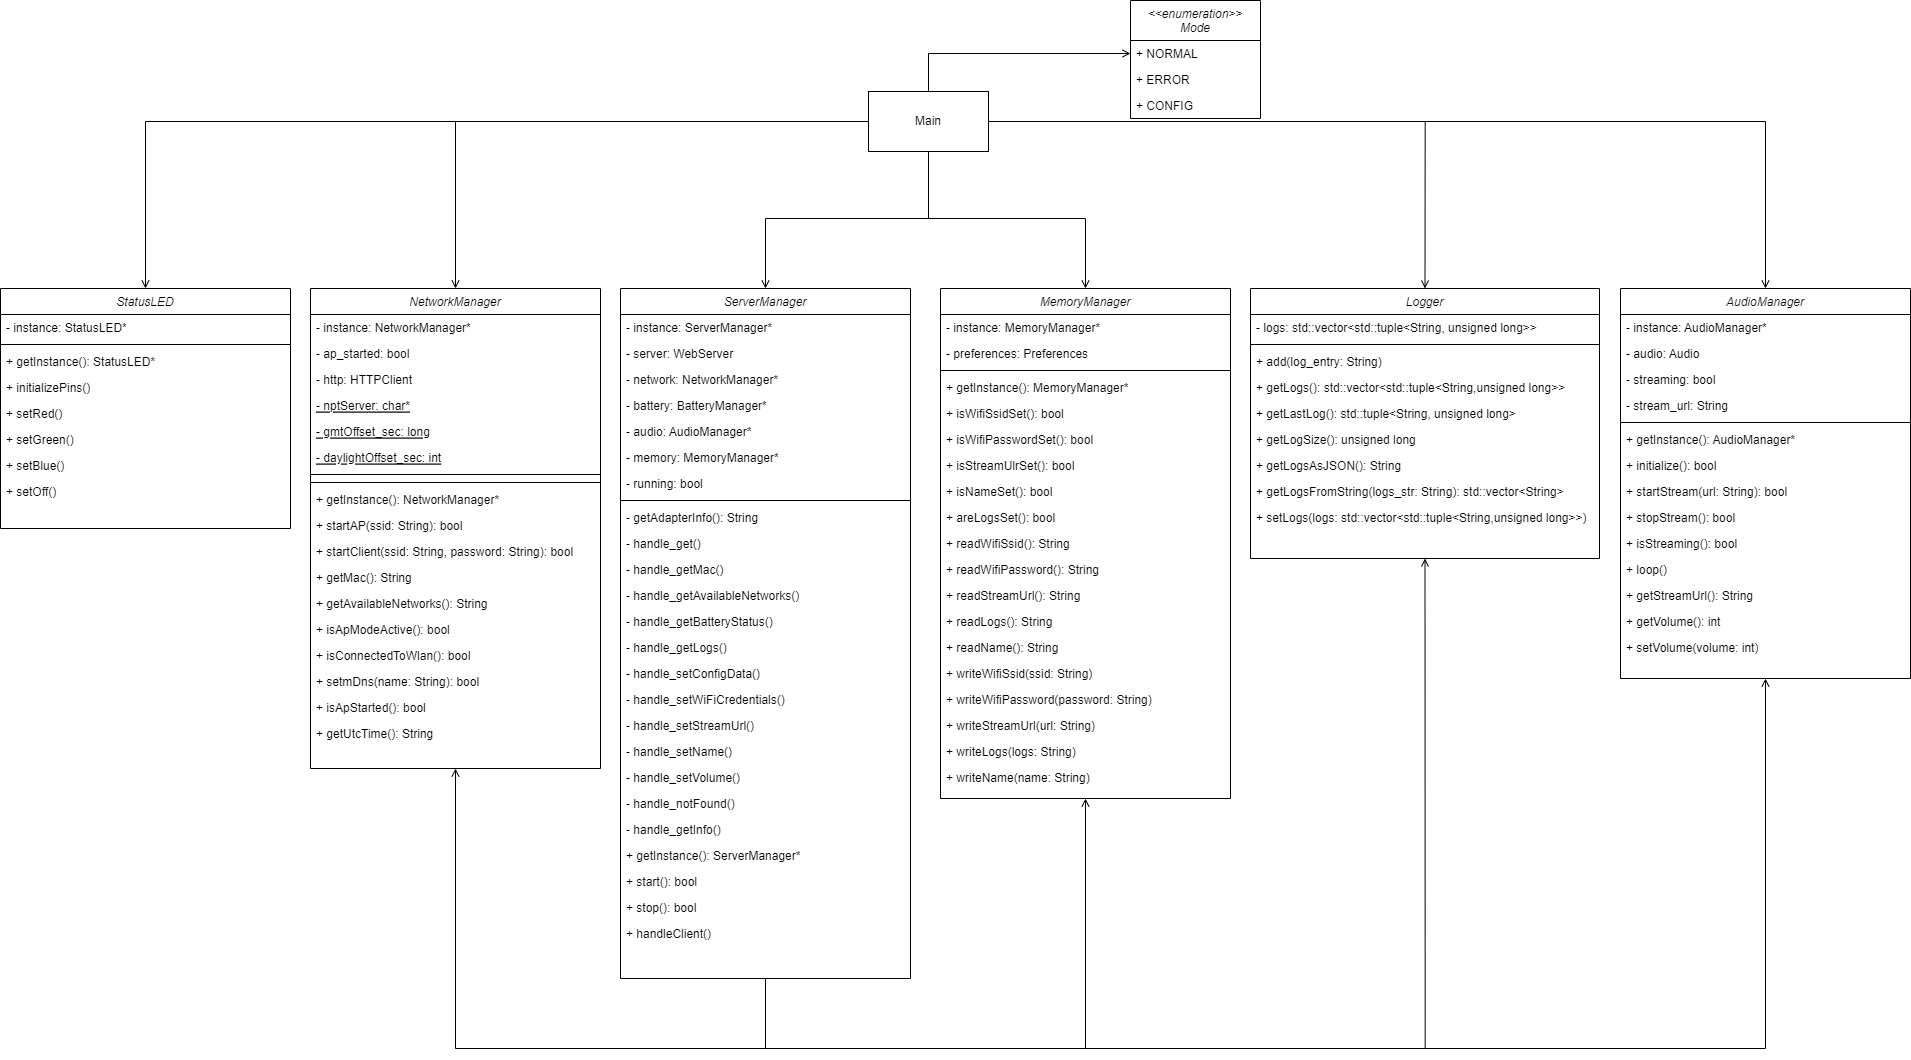
\includegraphics[scale=0.3, angle=90]{/software/uml_microcontroller.png}
\caption{UML-Klassendiagramm Microcontroller}
\end{figure}
\textbf{Mode} \\
Im ENUM Mode werden die verschiedenen Modi der Software definiert. Ein ENUM ist wie eine Art Datentyp, der Konstanten definiert, welche man verwenden darf. (vgl. URLPI15)  In unserem Fall definiert der ENUM die drei Modi NORMAL, CONFIG und ERROR. Diese geben den Status des Microcontrollers an. Der Modus NORMAL signalisiert, dass sich der Microcontroller im normalen Ablauf befindet. Im Modus CONFIG fungiert der Microcontroller als Access Point. Somit können sich Clients mit diesem verbinden und Konfigurationsdaten, wie WLAN-Anmeldedaten und Microcontroller-Name senden. Der Modus ERROR wird gesetzt, wenn ein Fehler im Programm auftritt. Dies ist zum Beispiel der Fall, wenn die Verbindung mit dem WLAN-Netzwerk nicht möglich ist. \newline \\
\textbf{StatusLED} \\
Mithilfe der Klasse StatusLED wird die RGB-LED, welche am Microcontroller angeschlossen ist, gesteuert. Mit ihr wird der aktuelle Modus des Microcontrollers angezeigt. Die nachstehende Tabelle beschreibt welche Farbe für welchen Modus steht: \newline \\
\begin{figure}[H]
\begin{tabular}{|l|l|}
\hline
\textbf{Modus} & \textbf{Farbe} \\
\hline
NORMAL & Grün \\
\hline
CONFIG & Blau \\
\hline
ERROR & Rot \\
\hline
\end{tabular}
\caption{Status-Farben}
\end{figure}
\textbf{NetworkManager} \\
Die Klasse NetworkManager kümmert sich um alle Funktionen, die mit dem WiFi des ESP32 zu tun haben. Es ist hier möglich den Access Point - Modus bzw. den Client-Modus zu aktivieren, sowie nach verfügbaren Netzwerken zu suchen und die MAC-Addresse des Adapters zu lesen. Diese Funktionen werden alle mithilfe der WiFi-Bibliothek verwirklicht.
\vspace{4mm}\newline
\textbf{AudioManager} \\
Die Klasse AudioManager ist für das Empfangen des Internet-Audio-Streams, für das dekodieren und für die Ausgabe der Audio-Signale zuständig. Dafür wird größtenteils die ESP32-I2SAudio Bibliothek verwendet.
\vspace{4mm}\newline
\textbf{Logger} \\
Die Klasse Logger ist für die Verwaltung von Logs, welche von anderen Klassen geschrieben werden, zuständig. In ihr ist ein Vektor, welcher Tuples, bestehend aus Log-Text und Log-Zeitpunkt, speichert, definiert. Diese Logs sind essentiell für die Fehlerbehebung, da man sehen kann welche Aktionen im Programm ausgeführt wurden. Die Klasse bietet Funktionen zum Hinzufügen von Logs und zum Anzeigen bestehender Logs. Die Funktionen sind alle statisch, das heißt man muss kein Objekt dieser Klasse erzeugen, um die Funktionen auszuführen.
\vspace{4mm}\newline
\textbf{ServerManager} \\
Die Klasse ServerManager ist für das Verwalten des Webservers, welcher auf dem Microcontroller läuft, zustängig. In ihr werden die Funktionen, welche durch die Aufrufe der REST-API ausgeführt werden, definiert. Die Kernfunktionen der Klasse werden vorallem durch die WebServer-Bibliothek bereitgestellt.
\vspace{4mm}\newline
\textbf{MemoryManager} \\
Die Klasse MemoryManager ist für das Schreiben in und das Lesen vom EEPROMs des Microcontrollers zuständig. Um das zu erreichen, wird die Preferences-Bibliothek verwendet. \newline \\
\textbf{BatteryManager} \\
Die Klasse BatteryManager regelt den Ladevorgang des ESP32 und liest den Akkustand aus.
\subsubsection{Programmablauf}
Da die arduino-esp32-Bibliothek verwendet wurde ist der Programmablauf gleich wie bei einem standardmäßigen Arduino-Programm. Ausgeführt wird das Main-File welches aus der Funktion setup() und der Funktion loop() besteht. Die Funktion setup() wird beim Start des Microcontrollers einmalig ausgeführt. Anschließend wird die Funktion loop() in einer Endlosschleife ausgeführt. Wenn also das Ende der Funktion loop() erreicht wird, fängt diese wieder von vorne an. Im folgenden Teil wird der Ablauf innerhalb den einzelnen Funktionen genauer beschrieben. \newline \\
\textbf{Setup} \\
\begin{figure}[H]
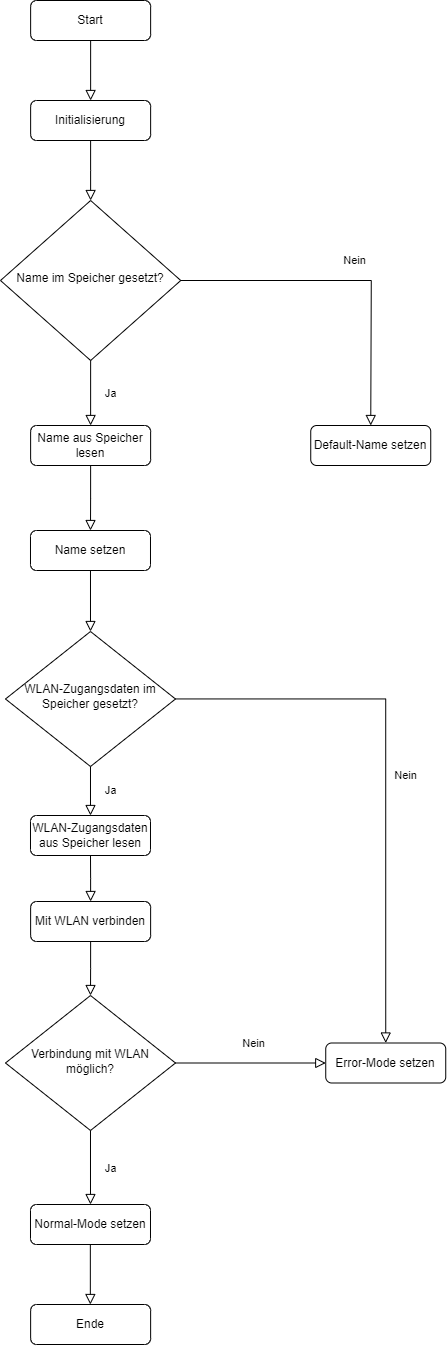
\includegraphics[scale=0.5]{/software/uml_ablauf_esp32_setup.png}
\caption{UML-Ablaufdiagramm Microcontroller Setup}
\end{figure}
Im Setup werden zuerst Konstanten, welche später im Programm benötigt werden, definiert. Auch werden am Anfang die entsprechenden Singleton-Klassen instanziert. Anschließend wird mithilfe der Klasse MemoryManager überprüft ob ein Name im EEPROM gesetzt ist. Ist dies der Fall, so wird der Name lokal als Variable gesetzt. Ist der Name allerdings nicht im EEPROM vorhanden, wird der Default-Name verwendet. Der Default-Name setzt sich zusammen aus MSA (kurz für Multiroom Sound Adapter) und den letzten zwei Stellen der Mac. Er ist somit für jeden Adapter eindeutig. Der Name wird später als SSID des Access Points bzw. für die mDNS verwendet. Nachdem der Name gesetzt ist, wird wiederum mit der Klasse MemoryManager überprüft ob WLAN-Zugangsdaten im EEPROM gespeichert sind. Sind die WLAN-Daten vorhanden so versucht der Microcontroller eine Verbindung mit dem gespeicherten WLAN herzustellen. Ist dies möglich wird der Modus auf Normal gesetzt. Ist dies nicht möglich bzw. sind keine WLAN-Zugangsdaten gespeichert, wird der Modus auf Error gesetzt. \newline \\
\textbf{Loop} \\
\begin{figure}[H]
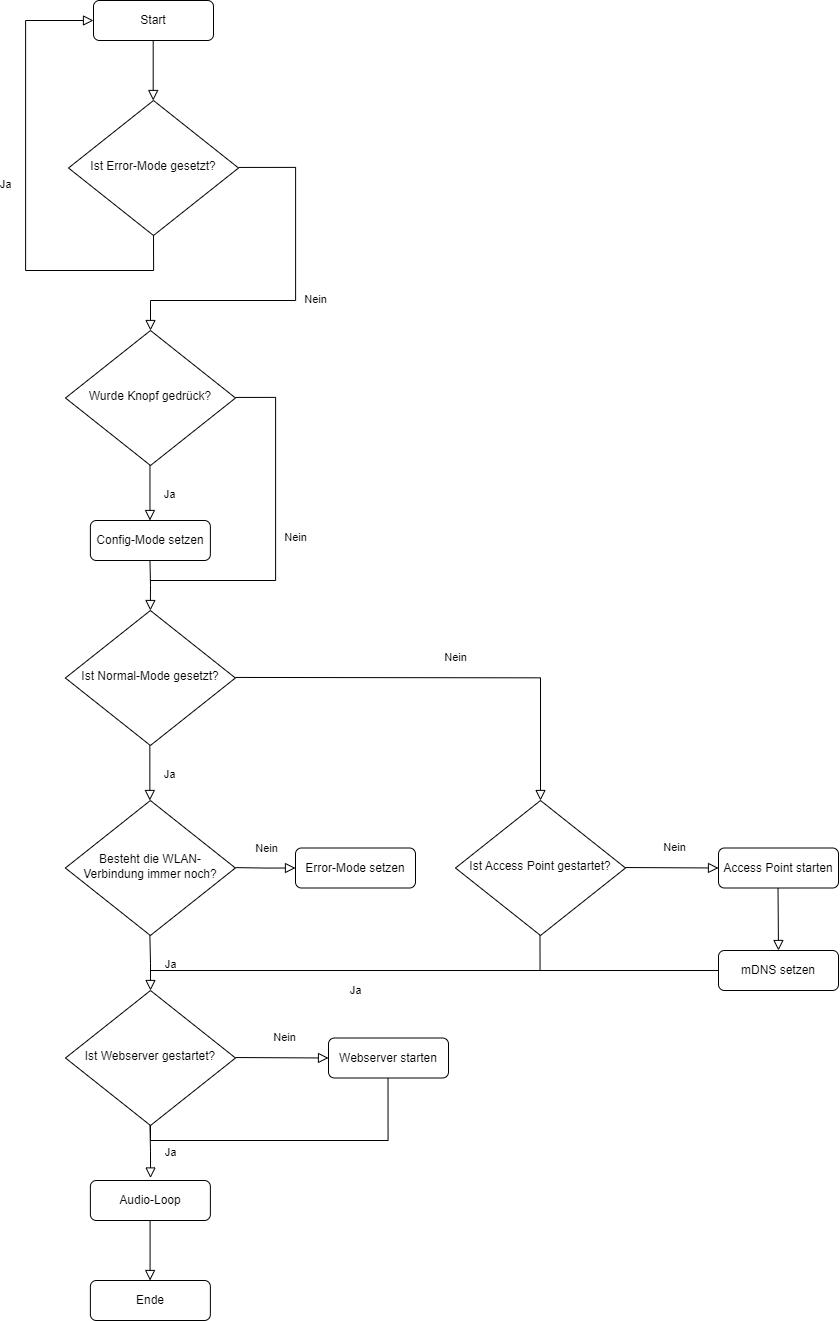
\includegraphics[scale=0.5]{/software/uml_ablauf_esp32_loop.png}
\caption{UML-Ablaufdiagramm Microcontroller Loop}
\end{figure}
Am Anfang der Loop-Funktion wird abgefragt ob der Modus auf Error gesetzt ist. Ist dies der Fall, wird nichts mehr ausgeführt, das heißt die Funktion springt wieder an den Startpunkt. Ist der Modus allerdings nicht auf Error gesetzt, wird überprüft ob der Knopf gedrückt ist. Wird dieser gedrückt, wird der Modus auf Config gesetzt. Anschließend wird überprüft ob der Modus auf Normal gesetzt ist. Ist dies der Fall wird überprüft ob immer noch eine Verbindung mit dem WLAN besteht. Dies geschieht mithilfe der Klasse NetworkManager. Wenn dies wahr ist, wird mithilfe der Klasse ServerManager überprüft ob der Webserver läuft. Wenn nicht, wird dieser gestartet. Ist der Modus allerdings nicht auf Normal gesetzt, also auf Config, so wird zuerst überprüft ob der Access Point gestartet ist. Wenn nicht, wird dieser schließlich gestartet und die mDNS wird gesetzt. Diese Prozesse werden wieder mithilfe der NetworkManager-Klasse durchgeführt. Anschließend wird ebenfalls der Zustand des Webservers überprüft. Am Schluss der Loop-Funktion wird noch die Funktion loop() der Klasse Audio-Manager ausgeführt. Diese regelt das Audio-Streaming.
\subsubsection{Erweiterungsmöglichkeiten}
In Zukunft sind noch weitere Funktionalitäten für die Software geplant. Im Hinblick auf die Sicherheit wäre es durchaus sinnvoll, den Webserver des Microcontrollers auf HTTPS umzustellen. Somit wäre eine verschlüsselte Kommunikation mit diesem möglich. Zusätzlich wäre es auch denkbar eine Funktion zu implementieren, die es ermöglicht mehrere Adapter zu Gruppen zu verbinden. In diesen Gruppen soll dann jeweils der gleiche Audio-Stream synchron empfangen und ausgegeben werden. Die Synchronisierung der Adapter bringt aber eine hohe Komplexizität mit sich, da man per WLAN-Verbindung mit sehr großen Latenzen zu rechnen hat. Ein Ansatz wäre zum Beispiel, dass jeder Microcontroller in einem bestimmten Intervall die Zeit von einem NTP (Network Time Protocoll) - Server abfragt und somit auf allen Microcontrollern die Zeit annähernd gleich ist. Dann könnte man die Buffer, welche vom Audio-Stream erhalten werden, mit einem Zeitstempel versehen und sie beim Erreichen dieser Zeit abspielen. Das Hauptproblem dieser Lösung wäre, dass die Zeitdifferenz zwischen den Microcontrollern vermutlich zu groß wäre und somit eine hörbare Latenz entsteht.
\subsection{Entwicklung Smartphone-App}
In diesem Kapitel wird der Übergang der Planung in die Entwicklung der Smartphone-App beschrieben.
\subsubsection{Zielsetzung}
Es wurde festgelegt, dass die Smartphoneapp folgende Anforderungen erfüllen soll:
\vspace{4mm}\newline 
\textbf{Verwalten von Adaptern}  \\
Mit der App soll es einerseits möglich sein, neue Adapter zu konfiguieren, andererseits, bereits hinzugefügte Adapter zu verwalten. Dabei können von den Adaptern verschiedene Daten, wie z.B. Akkustand und MAC-Adresse eingesehen werden.
\vspace{4mm}\newline
\textbf{Verwalten von Radiostationen} \\
Mit der App soll es außerdem möglich sein, nach Audiostreams von Internetradios zu suchen, und diese in einer Favoritenliste zu verwalten. \newline \\
\textbf{Verwalten von Verbindungen} \\
Mit der App soll es letztendlich möglich sein, eine Verbindungen zwischen Adaptern und Internetradio-Streams herzustellen und diese zu verwalten.
\subsubsection{Klassen}
In der App wurden folgende Klassen definiert: \newline \\
\textbf{Adapter} \\
Die Adapter-Klasse wird zum Erstellen von Adapter-Objekten verwendet. Sie definiert die Attribute, welche jeder Adapter haben muss. Dazu zählen Name, MAC-Addresse, eingestellte Lautstärke des Audio-Moduls, Erreichbarkeit und Akkustand. Diese Objekte werden in der App verwendet, um einfach mit den Daten der Adapter zu arbeiten. \newline \\
\textbf{Station} \\
Die Station-Klasse wird zum Erstellen von Station-Objekten verwendet. Sie definiert die Attribute, welche jede Radiostation haben muss. Dazu zählen Name, UUID, Icon-URL und Stream-URL. Das verwenden der Station-Objekte erleichtert die Handhabung von Stationen in der App. \newline \\
\textbf{Connection} \\
Die Connection-Klasse wird zum Erstellen von Connection-Objekten verwendet. In ihr wird ein Objekt der Klasse Adapter und ein Objekt der Klasse Station gespeichert. Damit wird die Verbindung zwischen Adapter und Station ersichtlich. Also welcher Adapter empfängt aktuell welchen Radiostream. \newline \\
\subsubsection{Funktionen}
In der Datei Utilities wurden Funktionen definiert, welche dabei helfen Daten abzurufen bzw. zu speichern. Dazu gehören Abfragen der RadioBrowser-API, Abfragen an den jeweiligen Adapter und Zugriffe in den Speicher. Speicheroperationen wurden mithilfe der in Expo integrierten Bibliothek \glqq AsyncStorage \grqq{}  durchgeführt. Abfragen mittels HTTP wurden mit der ebenfalls in Expo integrierten Bibliothek \glqq Axios \grqq{} durchgeführt. \newline \\
\textbf{Asynchrone Funktionen} \\
Alle der Funktionen in der Utilities-Datei wurden als asynchrone Funktionen deklariert. Asynchrone Funktionen werden immer dann verwendet, wenn eine Funktion ein Ergebnis nicht direkt beim Aufruf liefern kann, sondern dies noch eine gewisse Zeit in Anspruch nimmt. Diese Verhaltensweise wird realisiert, indem die Funktion ein sogenanntes Promise-Objekt zurückgibt. In diesem Objekt sind Callback-Funktionen deklariert, welche je nachdem ob das Ergebnis verfügbar ist oder ein Fehler auftritt ausgeführt werden. Es gibt dabei die Callback-Funktion resolve(ergebnis), welche ausgeführt wird, wenn die Funktion das Ergebnis hat und die Funktion reject(fehler), welche ausgeführt wird, wenn in der Funktion ein Fehler auftritt. Das praktische dabei ist, dass man beim Aufruf einer asynchronen Funktion, hinten eine .then(function(result)) Funktion anhängen kann, welche erst ausgeführt wird, wenn das Ergebnis verfügbar ist. Man kann aber auch mit await warten, bis das Ergebnis verfügbar ist. Mit .catch(function(error)) kann man Fehler abfangen welche eventuell in der Funktion auftreten. \newline \\
\textbf{Liste von verfügbaren Ländern/Sprachen abrufen} \\
Mit der Funktion getCountries() ist es möglich alle verfügbaren Ländernamen der RadioBrowser-API abzufragen. Der GET-Request wird dabei mit Axios ausgeführt. Als Rückgabe liefert die Funktion einen Promise, welcher entweder ein String-Array oder null ist. Das String-Array ist gefüllt mit allen verfügbaren Ländernamen. Null wird dann zurückgelifert, wenn bei der Abfrage ein Fehler auftritt. Es gibt außerdem noch eine Funktion um alle Sprachen der RadioBrowser-API aufzurufen. Diese Funktion ist gleich aufgebaut, der einzige Unterschied liegt in der URL, welche abgefragt wird. Die Ländernamen und Sprachen werden später für die Filterung der Radiostationen benötigt. \newline \\
\textbf{Stationen abfragen} \\
Die Funktion getStations(language, country) fragt alle Radiostationen, welche in der übergebenen Sprache bzw. dem übergebenen Land verfügbar sind, von der RadioBrowser-API ab und gibt diese dann JSON-Objekt zurück. Wenn bei der Abfrage ein Fehler entsteht, wird null zurückgeliefert. \newline \\
\textbf{Liste von Elementen vom Speicher lesen} \\
Die Funktion getFavouriteStations() fragt die Favoritenliste von Radiostationen, welche im Speicher gespeichert ist, ab. Diese wird als Array aus Station-Objekten zurückgegeben. Wenn keine Favoriten im Speicher sind, wird wiederum null zurückgegeben. Die Funktion zur Abfrage der Liste von gespeicherten Adaptern heißt getAdapters() und ist gleich aufgebaut. Der einzige Unterschied liegt im Rückgabetyp. Hier wird nähmlich ein Array aus Adapter-Objekten zurückgegeben.
\newline \\
\textbf{Element zum Speicher hinzufügen} \\
Die Funktion addFavouriteStations(stationList) fügt eine Liste aus Stationen, welche als Array aus Station-Objekten übergeben wird, der gespeicherten Favoritenliste hinzu. Wenn noch keine Favoritenliste gespeichert ist, wird eine neue erstellt. Die Funktion zum Hinzufügen eines neuen Adapters heißt dementsprechend addAdapter(adapter) und erwartet als Parameter ein einzelnes Objekt der Klasse Adapter.
\newline \\
\textbf{Element vom Speicher entfernen} \\
Die Funktion removeFavouriteStation(uuid) entfernt die Station mit der übergebenen UUID von der gespeicherten Favoritenliste, wenn diese dort vorhanden ist. Die UUID wird bereits von der RadioBrowser-API mitgeliefert und hilft dabei, jede Station eindeutig zu identifizieren. Die Funktion zum Entfernen eines Adapters aus dem Speicher heißt removeAdapter() und erwartet die Mac-Addresse des zu entfernenden Adapters als Argument. Durch diese ist auch jeder Adapter eindeutig identifizierbar. \newline \\
\textbf{Liste im Speicher leeren} \\
Die Funktion clearFavouriteStationList() wird die Favoritenliste im Speicher geleert, das heißt es sind keine Favoriten mehr gespeichert. Die Funktion zum leeren der Adapter-List heißt clearAdapterList() und löscht die Liste aller konfigurierten Adaptern aus dem Speicher. \newline \\ 
\subsubsection{Style}
Bei Style des User Inferface der App wurde auf Übersichtlichkeit und wenig Komplexität gesetzt. Der/Die Benutzer/in soll sich in der App schnellstmöglich zurecht finden. Zusätzlich wurde ein modernes Design im Darkmode erstellt. Der globale Style wurde in der App unter constants festgelegt. Hier sind Farben und Stile für häuig verwendete Komponenten definiert. Die optische Anpassung der Komponenten erfolgt ähnlich wie bei CSS (Cascading Style Sheets) \newline \\
\textbf{Farben} \\
Bei der Farbauswahl wurden als Hauptfarben eher dünklere Farben verwendet, um den Darkmode zu realisieren. Im Kontrast zu diesen wurden noch zusätzlich eher knalligere Farben im Turquise-Ton verwendet, um
bestimmte Zustände zu signalisieren. Im folgenden ist eine Tabelle mit den verwendeten Farben und deren Farbcodes im Hex-Format: \\
\begin{figure}[H]
\begin{tabular}{|l|l|}
\hline
\textbf{Bezeichnung} & \textbf{Farbcode (hex)} \\
\hline
grey & \# 2B2C28 \\
\hline 
lightTurquoise & \# 7DE2D1 \\
\hline 
white & \# FFFAFB \\
\hline 
red & \# d90b0b \\
\hline 
lightGrey & \# 3e403a \\
\hline 
\end{tabular} 
\caption{App-Farben}
\end{figure}
\subsubsection{Struktur}
\begin{figure}[H]
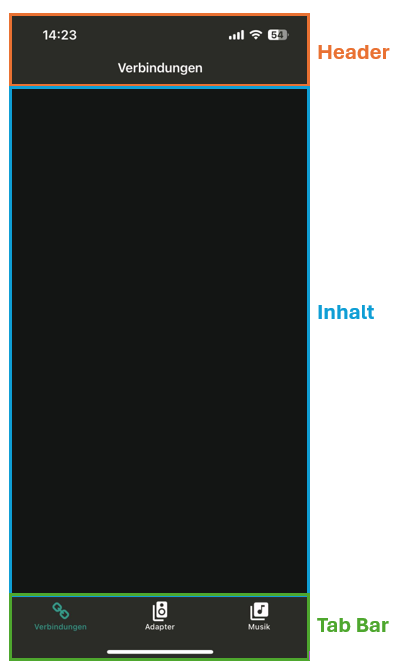
\includegraphics[scale=0.5]{/software/app_layout.png}
\caption{Aufbau Seite}
\end{figure}
Die Seiten der App sind alle gleich strukturiert. Ganz oben ist der Header, in welchem der Seitenname steht. Ganz unten ist die Tab Bar, welche die einzelnen Tabs anzeigt und auch sichtbar macht, in welchem Tab man sich aktuell befindet. Zwischen dem Header und der Tab Bar ist der jeweilige Inhalt der Seite.
Die App ist in drei Tabs gegliedert. Im folgenden werden die einzelnen Tabs genauer beschrieben. \newline \\
\textbf{Verbindungen} \\
Dieser Tab ist für die Verwaltung von Verbindungen zwischen Adaptern und Audioquellen zuständig. Hier kann konfiguriert werden, welcher Adapter welchen Stream empfangen soll. Es ist außerdem möglich, laufende Streams zu stoppen, deren Lautstärke zu ändern und zu löschen. \newline \\
\textbf{Adapter} \\
Dieser Tab ist für die Verwaltung von Adaptern zuständig. Es ist hier möglich, gespeicherte Adapter anzusehen, zu löschen und neue Adapter hinzuzufügen. Der Tab besteht aus den Seiten index und addAdapter, welche im Kapitel Seiten noch genauer beschrieben werden.  \newline \\
\textbf{Musik} \\
Dieser Tab ist für die Verwaltung von Audio-Quellen zuständig. Vorerst werden hier als Quellen nur Internet-Radios verwendet. In Zukunft wäre es aber auch denkbar, Streaming-Dienste als Quellen zu implementieren. Mit jetztigem Stand ist es in diesem Tab möglich, neue Radiosender zu der Favoritenliste hinzuzufügen und die Favoritenliste anzusehen bzw. Favoriten zu löschen. Der Tab besteht aus den Seiten index und searchStations, welche im Kapitel Seiten noch genauer beschrieben werden. \newline \\
\subsubsection{Navigation}
Für die Navigation in der App wurde einerseits die Tab-Navigation und andererseits die Stack-Navigation von Expo Router verwendet. Die App ist grundsätzlich in die drei Tabs Verbindungen, Adapter und Musik gegliedert. Zwischen diesen Tabs kann mittels dem Tab-Navigator gewechselt werden. In den einzelnen Tabs befinden sich jeweils mehrere Seiten. Diese Seiten sind mithilfe des Stack-Navigators aufrufbar. Der Stack-Navigator arbeitet mit einem sogenannten Stack, auf Deutsch \glqq Stapel \grqq{}. Zu diesem werden mittels des Last In - First Out - Prinzipes (kurz LIFO) Seiten hinzugefügt bzw. von diesem entfernt. Mithilfe der Methode router.push() werden dem Stack Seiten hinzugefügt. Es wird also sozusagen eine Seite auf den Stapel gelegt. Mithilfe der Methode router.pop() wird eine Seite vom Stack entfernt. Es wird also sozusagen die oberste Seite vom Stapel heruntergenommen.
\subsubsection{Komponenten}
In diesem Kapitel werden die selbst erstellen React-Komponenten genauer beschrieben. \newline \\
\textbf{AdapterItem} \\
Die Komponente AdapterItem wird dazu verwendet, die Daten eines einzelnen Adapters abzufragen und diese anzuzeigen. Dabei muss man dieser Komponente ein Objekt der Klasse Adapter als Argument mitgeben. Beim rendern wird direkt versucht eine Verbindung zum Webserver mit der IP-Adresse des übergebenen Adapters herzustellen. Ist dies erfolgreich, so wird ein GET-Request auf die /getInfo - Route des Adapters mittels Axios durchgeführt. Dabei werden die erhaltenen Informationen grafisch dargestellt. Zu diesen Daten zählt Lautstärke und Akkustand des Adapters. Ist der Adapter allerdings nicht erreichbar, werden die Daten nicht angezeigt. Gleichzeitig ändert sich die Hintergrundfarbe der Komponente zu einem helleren Grauton und es erscheint rechts eine durchgestrichene Wolke. Dies soll signalisieren, dass der Adapter nicht erreichbar ist. Diese Informations-Abfrage wird in einem Intervall von 5 Sekunden ausgeführt, um Änderungen in den Daten des Adapters bzw. der Verbindung des Adapters schnellstmöglich zu signalisieren. Dieses Intervall wird mit der JavaScript-Methode setInterval verwirklicht. Am Ende des renderns, wird das Interval noch geschlossen, um zu vermeiden, dass es mehrere Instanzen davon gibt. \newline \\
\textbf{AdapterList} \\
Die Komponente AdapterList stellt eine Liste dar, in der alle bisher hinzugefügten Adaptern aufgelistet sind. Die Adapter werden dabei mithilfe der AdapterItem-Komponente dargestellt. Die Adapter werden mithilfe der Methode getAdapter() aus dem Speicher abgefragt. Wenn noch keine hinzugefügten Adapter vorhanden sind bzw. die Methode getAdapter() null zurückgibt, wird die Komponente ErrorScreen dargestellt. \newline \\
\textbf{AddToListButton} \\
Die Komponente AddToListButton wurde verwendet, um ein drückbares Icon darzustellen, welches symbolisieren soll, ein weiteres Element zu einer Liste hinzuzufügen. Für die Umsetzung der Drück-Funktion wurde die Pressable-Komponente von React Native verwendet. Das Icon wurde von der Entypo-Bibliothek importiert. \newline \\
\textbf{BatteryIndicator} \\
Die Komponente BatteryIndicator zeigt die Batterieladung in Prozent mit dazugehörigem Icon an. Dabei erwartet sie als Argument die Batterieladung in Prozent. Je nachdem, in welchem Bereich diese Batterialadung liegt, wird ein entsprechendes Icon gerendert. Wenn für die Batterieladung ein negativer Wert (-1) übergeben wird, bedeutet dies, dass der Akku aktuell geladen wird. In diesem Fall, wird ein Lade-Icon dargestellt. \newline \\
\textbf{ConnectionItem} \\
... \newline \\
\textbf{DeleteButton} \\
Die Komponente DeleteButton stellt ein drückbares Icon dar, welches signalisieren soll, ein Element zu löschen. Dabei wurde die Drück-Funktion mit der Pressable-Komponente realisiert. Das Icon wurde von der FontAwesome-Bibliothek importiert. \newline \\
\textbf{ErrorScreen} \\
Die Komponente ErrorScreen stellt eine Ansicht bereit, die signalisieren soll, dass ein Fehler aufgetreten ist. Dabei wird die Fehlermeldung als Text angezeigt und man hat die Möglichkeit auf einen Knopf zu drücken, welcher dann eine Aktion ausführt. Als Parameter werden der zu anzeigende Text, der Text des Knopfs und die Funktion, welche beim druck auf den Knopf ausgeführt wird, übergeben. Der Fehlertext wird durch die Text-Komponente angezeigt und für den Knopf wurde eine Button-Komponnte verwendet. \newline \\
\textbf{FavouriteStationList} \\
Die Komponente FavouriteStationList stellt eine Liste aus mehreren StationItem-Komponenten dar. Die Daten dafür, werden beim Rendern der Komponente mithilfe der Funktion getFavouriteStations() aus dem Speicher ausgelesen. Wenn noch keine Favoriten im Speicher sind, wird die ErrorScreen-Komponente gerendert. Dabei ist es möglich, bei längerem Drücken auf ein FavouriteStationItem dieses zu selektieren und in weiterer Folge aus der Liste zu löschen. Die Selektierung wird mit einem kurzen Klick auf ein FavouriteStationItem wieder aufgehoben. Beim Druck auf die AddToListButton-Komponente, wird zum Screen "Stationsearch" navigiert. Beim druck auf die DeleteButton-Komponente, wird die ausgewählte Komponente aus dem Speicher gelöscht. \newline \\
\textbf{LoadingScreen} \\
Die Komponente LoadingScreen soll signalisieren, dass ein Vorgang durchgeführt wird und deshalb der Screen bzw. die Komponenten noch nicht angezeigt werden können. Dies kann zum Beispiel das Laden von Daten sein. Als Argument wird der Text übergeben, welcher in der Komponente angezeigt wird. Der Ladevorgang wird mit der ActivityIndicator-Komponente siganlisiert. \newline \\
\textbf{NetworkItem} \\
Die Komponente NetworkItem stellt Daten von einem Netzwerk dar. Dabei werden als Argumente die SSID und RSSI des Netzwerks übergeben. Die SSID wird mit der Text-Komponente angezeigt. Abhängig von dem Wert der RSSI werden verschiedene Icons angezeigt. Diese Icons stellen die Stärke des Netzwerks dar. Das Argument selected gibt an, ob die Komponente ausgewählt wurde. Wenn dies der Fall ist, verändert sich die Hintergrundfarbe der Komponente. \newline \\
Die Komponente StationItem stellt Name und Icon einer Radiostation dar. Die Radiostation wird dabei bei den Argumenten, als Objekt der Klasse Station übergeben. Das Argument selected gibt an, ob die Station ausgewählt ist. Wenn dies der Fall ist, verändert sich die Hintergrundfarbe der Komponente. \newline \\
\textbf{TextInputWindow} \\
Die Komponente TextInputWindow ermöglicht es Text in einem Fenster, welches vor dem anderen Content gerendert wird, einzugeben. Dabei ist unter dem Text ein Knopt "Bestätigen" und ein Knopt "Abbrechen" verfügbar. Der Text, welcher ganz oben angezeigt wird, wird als Argument übergeben. Außerdem wird mit isPassword festgelegt, ob die Eingabe in das Textfeld sichtbar sein soll oder nicht und die übergebenen Funktionen onEnter bzw. onCancel bestimmen, was passiert, wenn man den "Abbrechen"- oder "Bestätigen" Knopf drückt. \newline \\
\textbf{VolumeIndicator} \\
Die Komponente VolumeIndicator zeigt eine Lautstärke in Prozent an, mit einem Lautstärke-Icon davor. Das Lautstärke-Icon wird von der Feather-Bibliothek importiert. Die Lautstärke in Prozent wird mit einer Text-Komponente angezeigt. Als Argument wird die Lautstärke in Prozent übergeben. Wenn diese kleiner als 0 ist, wird ein Icon angezeigt, welches symbolisiert, dass die Lautstärke stumm ist. \newline \\
\textbf{WifiItem} \\
Die Komponente WiFiItem dient dazu, die Informationen eines WLAN-Netzwerkes darzustellen. Zu diesen Informationen zählt die SSID, welche sozusagen der Name des Netzwerks ist und die RSSI, welche die Stärke des Netzwerks angibt. Diese zwei Werte werden als Parameter der Komponente übergeben.
\subsubsection{Seiten}
In diesem Kapitel werden die einzelnen Seiten der App genauer beschrieben. \newline \\
\textbf{Startseite Verbindungen} \\
Diese Seite ist die Startseite des Tabs Verbindungen. Auf ihr werden aktive Verbindungen zwischen Adaptern und Audio-Quellen angezeigt. Die Darstellunge wird mithilfe der Komponente ConnectionList verwirklicht. Es ist hier möglich neue Verbindungen zu erstellen, aktive Verbindungen zu trennen, die Lautstärke von aktiven Verbindungen zu ändern und aktive Verbindungen zu pausieren bzw. fortzusetzen. \newline \\
\textbf{Verbindung hinzufügen} \\
Diese Seite befindet sich im Tab Verbindungen. Hier ist es möglich neue Verbindungen hinzuzufügen. Dazu muss zuerst ein Adapter ausgewählt werden und in weiterer Folge eine Audio-Quelle, von der der Adapter den Stream empfangen soll. Dabei können nur verbundene Adapter, das heißt, Adapter die im Netz erreichbar sind, ausgewählt werden. Zum Anzeigen der Adapter wurde die Komponente AdapterList verwendet, zum Anzeigen der Stationen die Komponente Station List. Der Parameter editable wurde dabei bei beiden Stationen auf false gesetzt, da ein bearbeiten der Listen in dieser Ansicht nicht möglich sein soll. Wenn jeweils ein Adapter und eine Station ausgewählt ist, ist es möglich den Knopf unten zu drücken und die Verbindung wird erstellt. \newline \\
\textbf{Startseite Adapter} \\
Diese Seite ist die Startseite des Tabs Adapter. Auf ihr werden hinzugefügte Adapter angezeigt. Dies geschieht mithilfe der Komponente AdapterList. Der Parameter editable der AdapterList hat den Wert true, da es hier möglich sein soll neue Adapter hinzuzufügen bzw. bestehende Adapter zu entfernen. \newline \\
\textbf{Startseite Musik} \\
Diese Seite ist die Startseite des Tabs Musik. Auf ihr werden die Favoriten der Radiostationen mithilfe der Komponente StationList dargestellt. Der Parameter selectable der StationList-Komponente hat dabei den Wert true, da es auf dieser Seite möglich sein soll, neue Favoriten hinzuzufügen bzw. bestehende Favoriten zu entfernen. In Zukunft wäre denkbar, dass hier noch Streaming-Dienste implementiert werden, welche dann auch als Audio-Quelle benutzt werden können. \newline \\
\textbf{Stationen filtern} \\
Diese Seite befindet sich im Tab Musik. Hier ist es möglich Land und Sprache auswählen, nach denen in weiterer Folge die Stationen auf der Seite Stationen auswählen gefiltert werden. Der Sprachen-Datensatz wird dabei mithilfe der Methode getLanguages() von Utilities abgerufen. Der Länder-Datensatz wird mit der Methode getCountries() von Utilities aufgerufen. Mit druck auf den Knopf wird die Seite Stationen auswählen aufgerufen und die Paramter werden an diese übergeben. \newline \\
\textbf{Stationen auswählen} \\
Diese Seite befindet sich im Tab Musik. Hier ist es möglich Stationen, welche zu der Favoritenliste hinzugefügt werden sollen, auszuwählen. Als Parameter werden Ländername und Sprache übergeben. Dementsprechend werden die zu auswählenden Stationen nach diesen Parametern gefiltert. Das Abrufen der Stationen erfolgt mithilfe der Methode getStations() und die Darstellung mithilfe der StationList-Komponente. Nach klick auf den Haken rechts unten werden die Stationen mithilfe der Funktion addFavouriteStations() zur Favoritenliste hinzugefügt. \newline \\
\textbf{Favoriten-Auswahl} \\
Auf dieser Seite wird eine Liste, mit allen Stationen, welche dem ausgewählten Land und der ausgewählten Sprache entsprechen, angezeigt. Hier kann man Radio-Stationen markieren und mit klick auf den Haken diese zu seiner Favoritenliste hinzufügen. \newline \\
\subsection{Design Adaptergehäuse}
Das Adaptergehäuse trägt einen wesentlichen Teil zur Sicherheit des Endverbrauchers sowie zur optimalen Funktionalität der Komponenten bei. Zudem soll es möglichst kompakt sein.
\subsubsection{Grundsätzlicher Aufbau}
Die Grundlage für den Prototyp bildet ein Kasten mit Deckel.\newline
Das Gehäuse wurde mit frei schwebenden, jedoch an den Wänden befestigten Stützen ausgestattet, um den Mikrocontroller fest montieren zu können. Der Prototyp wurde zudem mit kleinen Zylindern auf den Stützen ausgestattet, um den Mikrocontroller mit seinen bereits Vorhandenen Aussparungen darauf platzieren zu können. Der Digital-/Analogwandler und der Akku-Laderegler finden auch auf solchen Stützen ihren Platz. Der Gedanke dahinter war, den Akku unter den Bauteilen zu platzieren. Mehr dazu im Teil "Wärmeableitung". Zudem wurden in einer Wand des Gehäuses Aussparungen für die Buchsen platziert. Die Aussparungen für die RGB-LED und den Taster wurden im Deckel platziert. Eine Art Abdeckung für den Taster selbst wird auf diesen geklebt um ein gleichbleibendes Erscheinungsbild des Gehäuses zu behalten. Der Deckel, der von oben auf das Gehäuse gedrückt wird, schließt dieses. Im Deckel ist zusätzlich ein Belüftungsgitter eingelassen.
\subsubsection{Wärmeableitung}
Wärmeableitung ist wichtig, da Mikrocontroller, wie alle anderen Prozessoren auch, bei intensivem Betrieb Hitze entwickeln. Laut einer eigens durchgeführten Messung wird der in diesem Fall eingesetzte ESP32 meistens nur rund 38°C warm. Bei hoher Rechenleistung sind jedoch auch höhere Temperaturen möglich. Der ESP32 hat laut Hersteller eine mögliche Betriebstemperatur (Umgebungstemperatur) von –40°C bis +125°C. Damit die entstandene Wärme gut ableiten kann und keine der Komponenten stark beeinflusst (vor allem den Akku, da dieser bei hohen Temperaturen eine Explosionsgefahr darstellt), wird der Mikrocontroller im Gehäuse oben, also auf Stützen angebracht. Die aufsteigende Wärme kann somit nach oben durch das dafür vorgesehene Gitter entweichen und staut sich somit nicht im Inneren des Gehäuses. Der Akku liegt dementsprechend unter dem Mikrocontroller und allen anderen Komponenten und wird durch die abstrahlende Hitze dementsprechend nur etwas wärmer als Raumtemperatur.
\vspace{4mm}\newline
vgl. \url{https://www.espressif.com/en/products/socs/esp32}
\subsubsection{Virtuelles 3D-Design}
Um ein 3D-Modell des Prototypen zu zeichnen, wurde AUTODESK Fusion verwendet. Der Anbieter beschreibt seine Software folgendermaßen: "Autodesk Fusion verbindet Ihren gesamten Fertigungsprozess durch die Integration von CAD, CAM, CAE und PCB in einer einzigen Lösung, mit der Sie Ihre Ideen verwirklichen und praktisch alles fertigen können."\newline
Wenn man schon früh beachtet, dass die Prototypen mit einem 3D-Drucker gefertigt werden, kann man schon das 3D-Design für eine gute Druckbarkeit auf 3D-Drucker anpassen. Damit ist hauptsächlich gemeint, überhängende Drucke, komplizierte Stützstrukturen oder ähnliches zu vermeiden.
\vspace{4mm}\newline
\textbf{Basis} \newline
Die Basis des Adapters bildet ein 71x58x27mm großer Kasten mit 2mm Wanddicke. Aus Erfahrung kann man sagen, dass diese Dicke bei 3D-Drucken stabil ist, während sie jedoch nicht zu klobig wirkt.\newline
Die Stützen des Mikrocontroller beginnen auf 11mm Höhe und sind auf einer Längenseite 6x6x5mm und auf der anderen 6,9x6x5mm groß. Sie sind jeweils mit einer oder zwei Seiten an der Wand der Basis und somit überhängend. Dies wird im Teil "Drucken des Prototyps/Stützstruktur" noch wichtig.\newline
\begin{figure}[H]
\begin{flushleft}
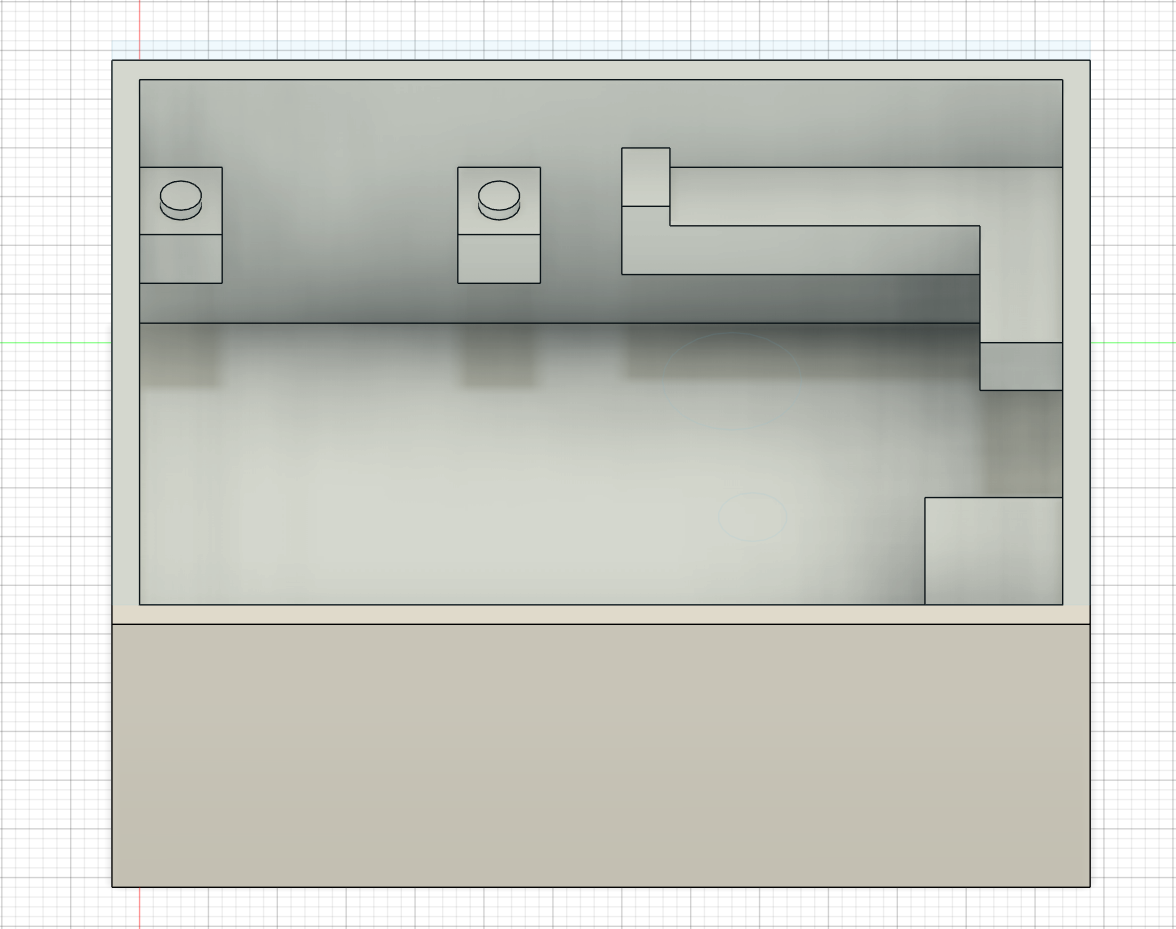
\includegraphics[scale=0.5]{/hardware/stuetzen_fusion.png}
\caption{Abbildung der Stützen für die Komponenten}
\end{flushleft}
\end{figure}
Auf den Stützen befinden sich jeweils Zylinder, die genau auf die Aussparungen des Mikrocontroller vermessen wurden. Die Zylinder haben einen Durchmesser von exakt 3mm. Der Abstand der Mittelpunkte dieser Zylinder war bei unserem Modell 47,10mm in der Länge und 23,10mm in der Breite. Auf einer Seite befindet sich zwischen Wand und Zylinder etwas mehr Platz, da der USB-C Port des Mikrocontrollers etwas über diesen herausragt. Deswegen auch der zuletzt erwähnte Versatz der Stütze von 0,9mm.\newline
Die Breite der Basis ist also genau auf die Länge von dem von uns benutzten Mikrocontroller zugeschnitten.\newline
In den gegenüberliegenden Ecken der Basis befinden sich der Digital-/Analogwandler und der Laderegler. Die Maße des Digital-/Analogwandler sind 31,8x17,2mm. Die Maße des Laderegler sind 28x17,45mm. Beide liegen, wie der Mikrocontroller auch, auf überhängenden, 5mm hohen Stützen auf. Aufgrund der USB-C Buchse wird der Halt des Laderegler noch von einer 3,5mm breiten 2mm-Erhöhung am Ende der Stütze verstärkt. Die USB-C Buchse wurde passend zum Laderegler und der Norm entsprechend (8,34x2,56mm Größe) eingelassen. Der Digital-/Analogwandler wird aufgrund der 3,5mm Klinkenbuchse von einer herabstehenden Wand gestützt, die im Teil "Deckel" genauer beschrieben wird. Die Aussparung der AUX-Buchse wurde auch passend für den Digital-/Analogwandler platziert und hat einen Durchmesser von 6mm.\newline
\begin{figure}[H]
\begin{flushleft}
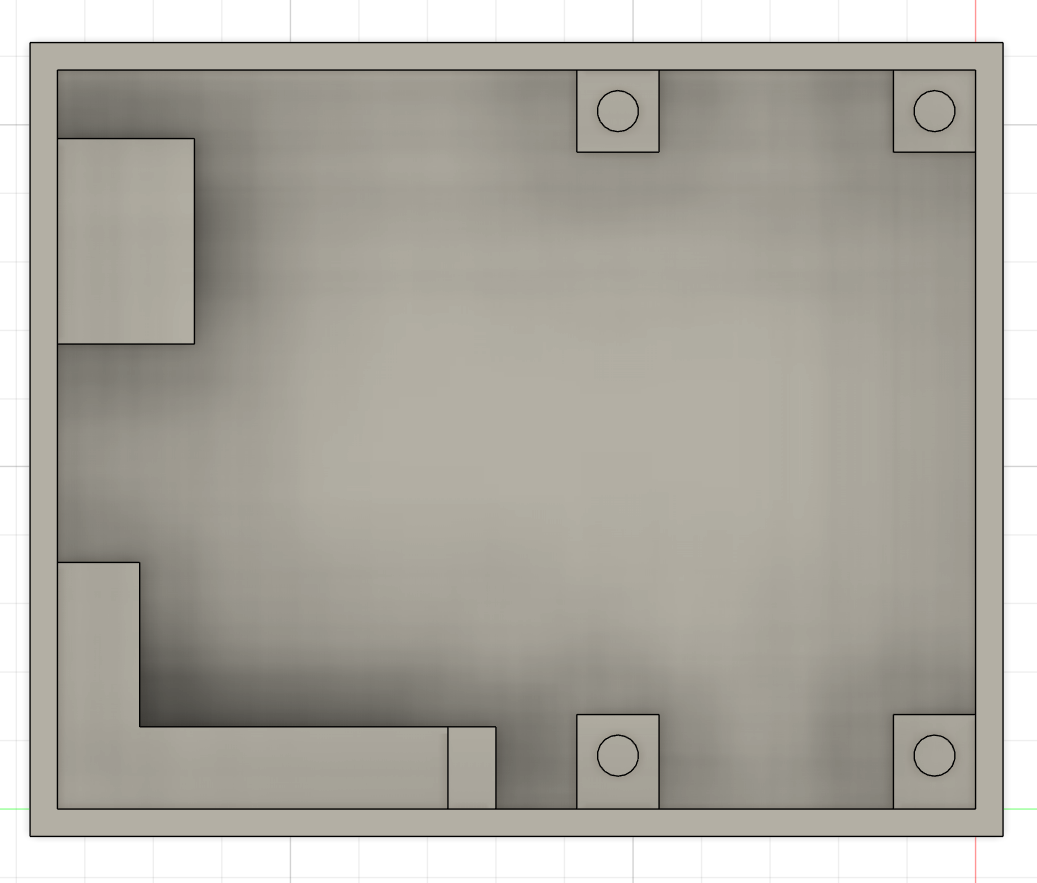
\includegraphics[scale=0.5]{/hardware/basis-draufsicht_fusion.png}
\caption{Draufsicht der Basis in AUTODESK Fusion}
\end{flushleft}
\end{figure}
\begin{figure}[H]
\begin{flushleft}
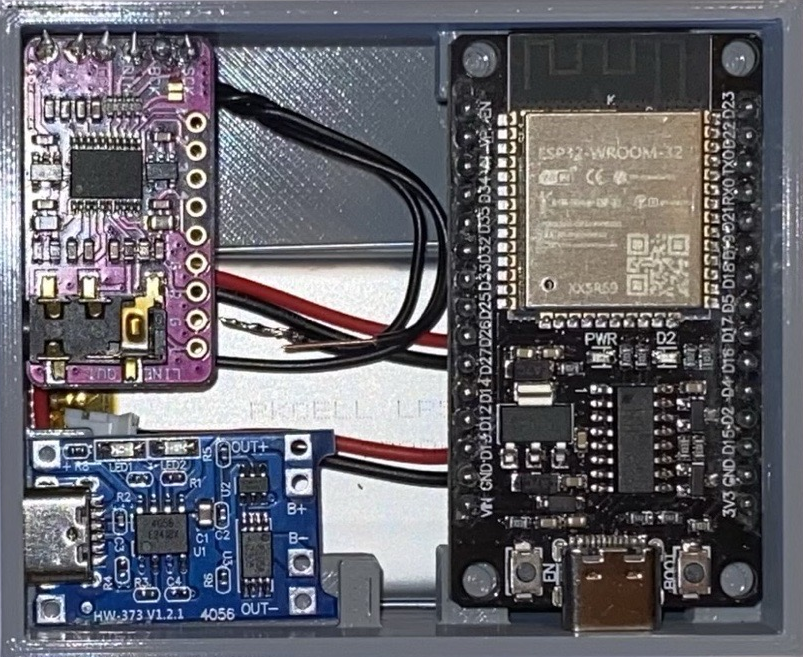
\includegraphics[scale=0.28]{/hardware/basis-inhalt_picture.png}
\caption{Bild der Basis mit den wichtigsten Komponenten an Ort und Stelle}
\end{flushleft}
\end{figure}
\vspace{4mm}
\textbf{Deckel} \newline
Der Deckel des Adapters ist grundsätzlich, wie die Wände der Basis, 71x58x2mm groß. Dieser hat jedoch eine zentrierte 67x54x1mm große Stufe. Mit dieser Stufe lässt sich der Deckel kleberlos auf den Adapter setzen und hält aufgrund der Eigenschaften des 3D-Drucks auch, zumindest für den Prototypen, fest genug.
Wie schon erwähnt, wird der DAW durch eine herabstehende Wand zusätzlich gestützt. Die Maße dieser Wand sind 32x2x10mm. Es würde keinen Sinn machen, die Wand wie beim Laderegler von der Außenwand aus überhängend zu machen, da der DAW länger als der Laderegler ist und die Buchse sich eher mittig in der entsprechenden Außenwand der Basis befindet.\newline
An der freien Seite der Stützwand (nicht die des DAW) befindet sich ein runder Schacht für die RGB-LED mit 5mm Durchmesser und eine Aussparung für den Aufsatz des Tasters mit 10,10mm Durchmesser. Der Taster mit den Grundmaßen 6x6mm wird durch eine Art U-Form aus Wänden im Gehäuse gehalten. Eine Wand davon bildet die gerade eben beschriebene Stützwand. Die untere Wand, auf der der Taster aufliegt, hat zudem zwei auf den Taster angepasste, 1mm große Aussparungen für die zwei Pole des Tasters.\newline
Wenn man in der Draufsicht auf den Deckel schaut, ist dort wo sich der Prozessor selbst befindet, ein Gitter in den Deckel eingelassen. Dieses Gitter hat die Maße 19,9x21,6mm, was etwas größer als der Prozessor des ESP32 ist. Das Gitter besteht aus diagonalen Streben, die jeweils 1,5mm breit sowie 1,5mm weit voneinander entfernt sind. So entsteht eine einfache und stabile Möglichkeit, Wärme durch den Deckel abzuleiten.\newline
\begin{figure}[H]
\begin{flushleft}
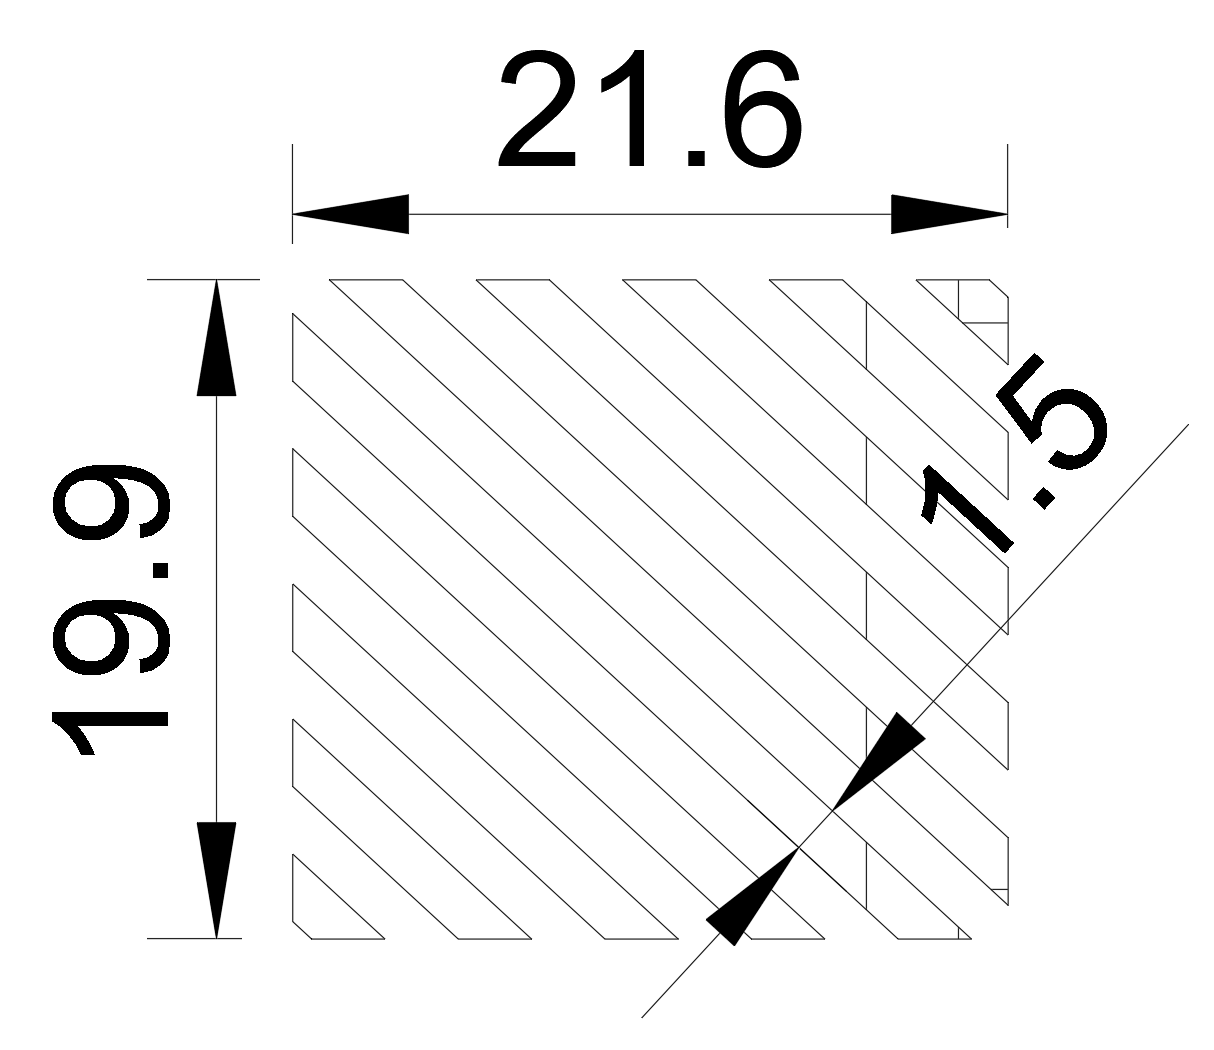
\includegraphics[scale=0.3]{/hardware/gitter-schema_fusion.png}
\caption{bemaßte Skizze des Belüftungsgitters in AUTODESK Fusion}
\end{flushleft}
\end{figure}
\vspace{4mm}
\textbf{Tasteraufsatz} \newline
Den Tasteraufsatz bildet ein Zylinder mit 9,5mm Durchmesser, auf dem sich ein weiterer Zylinder mit 5,5mm Durchmesser und zentrierter 3,5mm Aussparung für den Taster befindet.
\vspace{4mm}\newline
vgl. \url{https://www.autodesk.com/de/products/fusion-360/overview}\newline
vgl. \url{https://www.elektronik-kompendium.de/sites/com/2009021.htm}

\subsection{Fertigung Adaptergehäuse}
Das Material unseres Gehäuses wurde auf Kunststoff begrenzt. Für die Fertigung von Kunststoffgehäusen gibt es hauptsächlich diese Möglichkeiten (in diesem Fall kommt mangels Alternativen nur der 3D-Druck in Frage): 
\vspace{4mm}\newline
\textbf{Spritzgießen} \newline
\glqq Beim Spritzgießen wird der Kunststoff aus einem Plastifiziergerät (erwärmt den Kunststoff auf Schmelztemperatur) in einen Hohlraum (Formwerkzeug) gespritzt, in welchem er erst verdichtet wird und dann erkaltet.\grqq \newline 
Ein Vorteil für dieses Verfahren ist, dass auch komplizierte Formteile voll automatisiert sehr schnell in hohen Stückzahlen produziert werden können.
Der große Nachteil sind jedoch die hohen Stückkosten für die Formwerkzeuge.\vspace{4mm}\newline 
vgl. \url{https://www.chemie.de/lexikon/Kunststoffverarbeitung.html}
\vspace{4mm}\newline
\textbf{3D-Druck} \newline
Die zwei gängigsten 3D-Druck-Methoden sind Filament und Resin (Harz). Aufgrund des hohen Aufwands, den ein Resin-Drucker mit sich bringt, wurde für dieses Projekt die Methode mit Filament gewählt. \newline
Beim 3D-Drucken durch Fused Deposition Modeling (Schichtschmelzverfahren) wird Kunststoff in Drahtform (Filament) (die häufigsten Dicken sind 2,85mm (allgemein als 3mm bezeichnet) und 1,75mm wobei die 1,75mm Version weltweit am häufigsten verbreitet ist) durch beheizte Düsen geleitet und somit geschmolzen. Das nun weiche Filament wird in Schichten auf die Druckplatte aufgetragen und erhärtet kurz darauf. Durch dieses Schichten lassen sich präzise Körper aus Kunststoff bauen.
\vspace{4mm}\newline
vgl. \url{https://www.printer-care.de/de/drucker-ratgeber/wie-funktioniert-ein-3d-drucker}\newline
vgl. \url{https://help.prusa3d.com/de/glossary/175-mm_134816}

\subsubsection{Drucken des Prototypen}
Die Gehäuse-Prototypen wurden mit einem \glqq PRUSA MK4S\grqq{} 3D-Drucker gefertigt. Alle FFF-Drucker von Prusa sind grundsätzlich für 1,75-Filament konfiguriert.
\vspace{4mm}\newline
\textbf{Druckeinstellungen} \newline
Die Temperatur der Build Plate lag bei uns Standartmäßig auf 60°C. Die Drucktemperatur, also die der Nozzle (Düse) lag bei etwa 185°C. \newline
Das erste Layer wurde mit 0,15mm Dicke gedruckt, die restlichen mit 0,2mm Dicke. \newline
Als Infill-Pattern wurde \glqq Grid\grqq{} mit 20\% Dichte und 4mm Line-Distance gewählt. \newline
Das Drucken verlief mit den von uns gewählten Einstellungen reibungslos, jedoch an manchen Stellen etwas unsauber. Beispielsweise war das Ergebnis der Aussparung für den Taster im Deckel des Adapters so ungenau, dass der Durchmesser des Aufsatzes für den Taster um 0,5mm verkleinert werden musste. Sonstige Ungenauheiten stellten, zumindest abgesehen von der Optik, kein Problem dar. \newline
Man darf auch nicht vergessen, dass gewisse Drucke (Gehäusedeckel und -basis) Stützstrukturen erfordern. Stützstrukturen sind Konstruktionen, die der Drucker zur Unterstützung stark überhängender oder freischwebender Strukturen druckt. Jedoch sind diese nur temporär. Da das Stützmaterial nicht so fest an der Druckfigur haftet, wie die Teile der Figur selbst, kann es nach dem Druck mit einer herkömmlichen Zange entfernt werden. Diese Stützstrukturen lassen sich in der Slicer-Software genau einstellen und konfigurieren. So kann man unter anderem sicherstellen, dass das Entfernen einfach möglich ist und die Stützstruktur die Figur selbst nicht all zu stark beeinflusst.
\vspace{4mm}\newline
vgl. \url{https://help.prusa3d.com/de/glossary/175-mm_134816}
\subsection{Zusammensetzen des Prototypen}
Die Komponenten werden jeweils einzeln direkt mit dem Mikrocontroller verbunden. Bei diesem Prototyp lässt sich der Mikrocontroller nämlich vorerst als Platine betrachten, welcher zusätzliche Komponenten zugefügt werden.
\subsubsection{Schaltplan}
Die Verdrahtung zwischen den Komponenten und dem Mikrocontroller ist folgendermaßen gelöst:
\vspace{4mm}\newline
\textbf{Digital-/Analogwandler} \newline
BCK (Wandler) an D26 (Mikrocontroller)\newline
LCK (Wandler) an D25 (Mikrocontroller)\newline
DIN (Wandler) an D22 (Mikrocontroller)\newline
\vspace{4mm}\newline
\textbf{Taster} \newline
1 (Taster) an 3V3 (Mikrocontroller)\newline
2 (Taster) an D12 (Mikrocontroller)\newline
\vspace{4mm}\newline
\textbf{RGB-LED} \newline
R (LED) an D15 (Mikrocontroller)\newline
G (LED) an D2 (Mikrocontroller)\newline
B (LED) an D4 (Mikrocontroller)\newline
GND (LED) an GND (Mikrocontroller)\newline
\subsubsection{Verdrahten}
Bei unserem Prototypen wurden alle Komponenten, der Pinbelegung entsprechend, mit dem Mikrocontroller verbunden. Dabei kamen Drahtkabel, Litzenkabel und Steckkabel (herkömmliche Jumper Kabel) zur Verwendung. Dies hatte hauptsächlich den Grund, dass zum Beispiel nur mit Drähten nicht alle Verbindungen optimal möglich gewesen wären. Das ist hauptsächlich der Löthaftung an einigen Komponenten geschuldet. Um keine Wackelkontakte, oder gar unterbrochene Verbindungen zu riskieren, wurde für jede Verbindung einzeln entschieden, welches der genannten Verfahren sich am besten eignet. So entstanden zum Beispiel Steckverbindungen, gelötete Drahtverbindungen oder Mischungen aus gelöteten Litze- und Steckverbindungen (jeweils am anderen Ende des Kabels).
\vspace{4mm}\newline
\textbf{Löten}\newline
\glqq Das Löten ist das Verbinden von Metallteilen durch eine Metalllegierung (das Lot) unter Einfluss von Wärme/Hitze.\grqq{} \newline
Man unterscheidet grundsätzlich zwischen Weich- und Hartlöten. Ausschlaggebend dabei ist die Schmelztemperatur des Lots. So haben Weichlote eine Schmelztemperatur unter 450°C während Hartlote erst ab 450°C bis etwa 1100°C schmelzen. \glqq Das Weichlot wird verwendet, wenn die Verbindung zweier Metalle dicht und Leitfähig sein soll und um die mechanische Belastbarkeit keine hohe Anforderung gestellt wird. \grqq{} Da die in diesem Projekt benutzten Bauteile jedoch keine höheren Temperaturen vertragen, war Weichlöten für dieses Projekt die einzige Wahl. \newline
Um einen Lötvorgang aus eigener Erfahrung möglichst kurz zu beschreiben:\newline
Man hat beispielsweise zwei Kabel die man verbinden möchte und die Verbindung sollte möglichst fest halten und gut leiten. Zuerst müssen die Enden der Kabel abisoliert werden. Es kann helfen, wenn man die Enden schon vor der eigentlichen Verbindung sozusagen etwas \glqq verzinnt\grqq{}. Nun richtet man die Kabel zueinander so aus, wie sie später fixiert sein sollen. Man fährt mit dem Ende des Lots (umgangssprachlich Lötzinn) an die heiße Spitze des Lötkolben und schmilzt so etwas Lot auf die Verbindungsstelle (nicht zu viel, sonst erhält man dicke Tropfen; jedoch auch nicht zu wenig, da die Verbindung dann möglicherweise nicht ausreichend hält). Nach dem abkühlen macht es Sinn, die Lötverbindung durch leichtes rütteln oder ziehen zu überprüfen. Löten ist letztendlich aber ein Handwerk, das für saubere Ergebnisse Geduld und Übung vorraussetzt.
\vspace{4mm}\newline
(vgl. \url{https://www.elektronik-kompendium.de/sites/grd/0705261.htm})
\subsubsection{Kleben}
Damit alle Komponenten und Teile sicher im Gehäuse sitzen und nichts klappert oder sich gar bewegt, worunter die Lötverbindung leiden würde, müssen gewisse Komponenten angeklebt werden. Vorallem bei den Buchsen ist eine feste Verbindung wichtig, da diese bei jedem Ein- und Ausstecken großer Belastung ausgesetzt sind. Somit wurden der Laderegler und der Digital-/Analogwandler an den dafür gedruckten Stützen angeklebt. Zudem wurde der gedruckte Aufsatz in Gehäuseoptik für den Taster auf diesem befestigt. Für alle Klebverbindungen im Adapter wurden entweder herkömmliches Cyanacrylat (Superkleber) oder Schmelzklebstoff (Heißkleber) verwendet.

\section{Testen und Fehlerbehebung}
\subsection{Testen des Gesamtsystems}
\subsubsection{Testen des Prototypen}
Es gibt unzählbar viele Möglichkeiten einen Prototypen auf Herz und Nieren zu testen. Diese Diplomarbeit beschränkt sich jedoch auf einige wesentliche Aspekte wie Verarbeitung, Funktion und Useability.
\vspace{4mm}\newline
\textbf{Verarbeitung}
\vspace{4mm}\newline
Positives:\newline
Die äußere Verarbeitung des Multi Room Sound-Adapters ist für einen Prototypen sehr gut ausgefallen. Fertig zusammengesetzt wirkt das Gerät stabil und wertig. Es hat etwas Gewicht und nichts klappert wenn man es schüttelt. Die Buchsen halten der für Buchsen gemäßen Belastung stand. Beide der Buchsen lassen sich problemlos benutzen, beim Ein- und Ausstecken gibt es keine Probleme. Der Taster des Adapters ist, zumindest unseren Erwartungen nach, besonders gut ausgefallen, er hat ein angenehmes Klickfeeling und lässt sich reibungslos betätigen. Die Statusanzeige funktioniert so wie sie soll.

Negatives:\newline
Man sieht dem Gehäuse bei guter Beleuchtung eindeutig an, dass es 3D-gedruckt wurde. Manche Oberflächen wirken eher geriffelt als flach. Diese Oberflächeneigenschafen sind völlig normal für 3D-Drucker und beeinflussen die Funktionsweise des Gesamtsystems kaum. Bei einem tatsächlichen Vetrieb des Produkts müsste man sich jedoch noch einmal genau über Herstellungsmöglichkeiten für kleinere Gehäuse informieren oder das Gehäuse, wie auch bei der Auswahl des Fertigungsverfahrens schon kurz diskutiert, einfach Spritzgießen lassen. Ein Spritzguss hat bessere Oberflächeneigenschaften als ein 3D-Druck.
\vspace{4mm}\newline
(vgl. \url{https://2d-spritzguss.de/3d-druck-spritzguss})
\vspace{4mm}\newline
\textbf{Funktion}\newline
Der Adapter funktioniert und erfüllt seine Funktionen ohne Fehler oder Komplikationen.
\vspace{4mm}\newline
\textbf{Usability}\newline
Die Anwendung des Adapter ist grundsätzlich angenehm. Es gilt jedoch zu bedenken, dass uns sowohl Software als auch Hardware schon bekannt sind. Wie sich die Usability verändert, wenn der Adapter von jemandem benutzt wird, der ihn noch nie gesehen hat, kann man nur schlecht sagen. Dafür wären mehrere Produkttests nötig. Falls ein Vetrieb des Produkts in betracht gezogen werden würde, wäre dies auf jeden Fall ein wichtiger Punkt.\newline
\subsection{Auftretende Fehler beheben}
Es handelt sich hierbei nicht direkt um einen Fehler, jedoch ist uns wichtig, dass auch die Optik des Gehäuse so gut wie möglich ausfällt. Deshalb wurde viel mit verschiedenen Tricks und Methoden gearbeitet, die 3D-Drucke wertiger ausfallen zu lassen.\newline
So war anfangs beispielsweise die Druckgenauigkeit in Millimeter nicht auf dem kleinst-möglichen Wert, was für Testdrucks aufgrund der wesentlich kürzeren Druckzeit jedoch völlig in Ordnung ist. Wenn alles passt, macht es aber definitiv Sinn eine lange Druckdauer in Kauf zu nehmen, um das für den vorliegenden 3D-Drucker genauste Ergebnis zu erhalten.\newline
Eine Herausforderung war die Beschriftung des Deckels. Diese war beim ersten Testdruck teilweise unlesbar ungenau. Das der \glqq Boden\grqq{} der Schrift auf Grund des druckabhängigen Überhanges (die größte Fläche also die Oberseite des Deckels muss praktisch auf der Druckplatte sein) nicht glatt wird, war uns klar. Jedoch hatte dieses Erscheinungsbild augenscheinlich nichts mit dem Überhang zu tun. Bei genauerem Betrachten fiel auf, dass das erste Layer fast wie gepatzt aussah. Ein weiterer Versuch mit simpler Schriftart und bei dem lediglich die Druckgenauigkeit des ersten Layers von 0.15 auf 0.1, die der restlichen Layer von 0.2 auf 0.15 kalibriert wurde, zeigte jedoch schon für einen 3D-Druck schöne Ergebnisse.\newline
Eine weitere Möglichkeit zum glätten der schon zuvor beschriebenen riffelartigen Oberflächen ist sogenanntes Ironing. \glqq Ironing beschreibt die einstellbare Funktion in einiger Slicer-Software. Ironing bietet dir die Möglichkeit, die letzte 3D-Druckschicht mit der Nozzle zu "bügeln". Die Nozzle deines 3D-Druckers bewegt sich ohne dabei zu extrudieren nochmals über die zuletzt gefertigte Schicht. Durch diesen Vorgang glättet sie die Objekt-Oberfläche. Du bekommst somit eine verbesserte und glatte letzten Schicht.\grqq{} Beim PRUSA MK4S war diese Funktion sehr zufriedenstellend. Oberflächen werden, ohne den gesamten Druck zu beeinflussen, glatter.\newline
\vspace{4mm}\newline
(vgl. \url{https://www.3dprima.com/de/3dprima/tipps-tricks-begriffe-3d-druck#Ironing})
\subsection{Test auf Cybersecurity}
In diesem Kapitel wird der gesamte Code auf Sicherheitslücken getestet.
\subsection{Auftretende Sicherheitslücken schließen}
In diesem Kapitel werden die bei den Tests aufgetretenen Sicherheitslücken geschlossen.
\section{Einzelnachweise}
\subsection{Literaturverzeichnis}
\subsection{Abbildungsverzeichnis}
\listoffigures
\subsection{Anhang}
\subsubsection{Code Microcontroller}
\subsubsection{Code Smartphoneapp}
\end{document}